% Options for packages loaded elsewhere
\PassOptionsToPackage{unicode}{hyperref}
\PassOptionsToPackage{hyphens}{url}
%
\documentclass[
]{book}
\usepackage{lmodern}
\usepackage{amssymb,amsmath}
\usepackage{ifxetex,ifluatex}
\ifnum 0\ifxetex 1\fi\ifluatex 1\fi=0 % if pdftex
  \usepackage[T1]{fontenc}
  \usepackage[utf8]{inputenc}
  \usepackage{textcomp} % provide euro and other symbols
\else % if luatex or xetex
  \usepackage{unicode-math}
  \defaultfontfeatures{Scale=MatchLowercase}
  \defaultfontfeatures[\rmfamily]{Ligatures=TeX,Scale=1}
\fi
% Use upquote if available, for straight quotes in verbatim environments
\IfFileExists{upquote.sty}{\usepackage{upquote}}{}
\IfFileExists{microtype.sty}{% use microtype if available
  \usepackage[]{microtype}
  \UseMicrotypeSet[protrusion]{basicmath} % disable protrusion for tt fonts
}{}
\makeatletter
\@ifundefined{KOMAClassName}{% if non-KOMA class
  \IfFileExists{parskip.sty}{%
    \usepackage{parskip}
  }{% else
    \setlength{\parindent}{0pt}
    \setlength{\parskip}{6pt plus 2pt minus 1pt}}
}{% if KOMA class
  \KOMAoptions{parskip=half}}
\makeatother
\usepackage{xcolor}
\IfFileExists{xurl.sty}{\usepackage{xurl}}{} % add URL line breaks if available
\IfFileExists{bookmark.sty}{\usepackage{bookmark}}{\usepackage{hyperref}}
\hypersetup{
  pdftitle={Software Installation Guide},
  pdfauthor={Francisco Rowe, Dani Arribas-Bel},
  hidelinks,
  pdfcreator={LaTeX via pandoc}}
\urlstyle{same} % disable monospaced font for URLs
\usepackage{longtable,booktabs}
% Correct order of tables after \paragraph or \subparagraph
\usepackage{etoolbox}
\makeatletter
\patchcmd\longtable{\par}{\if@noskipsec\mbox{}\fi\par}{}{}
\makeatother
% Allow footnotes in longtable head/foot
\IfFileExists{footnotehyper.sty}{\usepackage{footnotehyper}}{\usepackage{footnote}}
\makesavenoteenv{longtable}
\usepackage{graphicx,grffile}
\makeatletter
\def\maxwidth{\ifdim\Gin@nat@width>\linewidth\linewidth\else\Gin@nat@width\fi}
\def\maxheight{\ifdim\Gin@nat@height>\textheight\textheight\else\Gin@nat@height\fi}
\makeatother
% Scale images if necessary, so that they will not overflow the page
% margins by default, and it is still possible to overwrite the defaults
% using explicit options in \includegraphics[width, height, ...]{}
\setkeys{Gin}{width=\maxwidth,height=\maxheight,keepaspectratio}
% Set default figure placement to htbp
\makeatletter
\def\fps@figure{htbp}
\makeatother
\setlength{\emergencystretch}{3em} % prevent overfull lines
\providecommand{\tightlist}{%
  \setlength{\itemsep}{0pt}\setlength{\parskip}{0pt}}
\setcounter{secnumdepth}{5}
\usepackage{booktabs}
\usepackage{amsthm}
\makeatletter
\def\thm@space@setup{%
  \thm@preskip=8pt plus 2pt minus 4pt
  \thm@postskip=\thm@preskip
}
\makeatother
\usepackage[]{natbib}
\bibliographystyle{apalike}

\title{Software Installation Guide}
\author{Francisco Rowe, Dani Arribas-Bel}
\date{2020-10-02}

\begin{document}
\maketitle

{
\setcounter{tocdepth}{1}
\tableofcontents
}
\hypertarget{purpose}{%
\chapter*{Purpose}\label{purpose}}
\addcontentsline{toc}{chapter}{Purpose}

This guide provides step-by-step description on how to install and access Python from your own computer.

Select your Operating System and follow the steps.

\begin{center}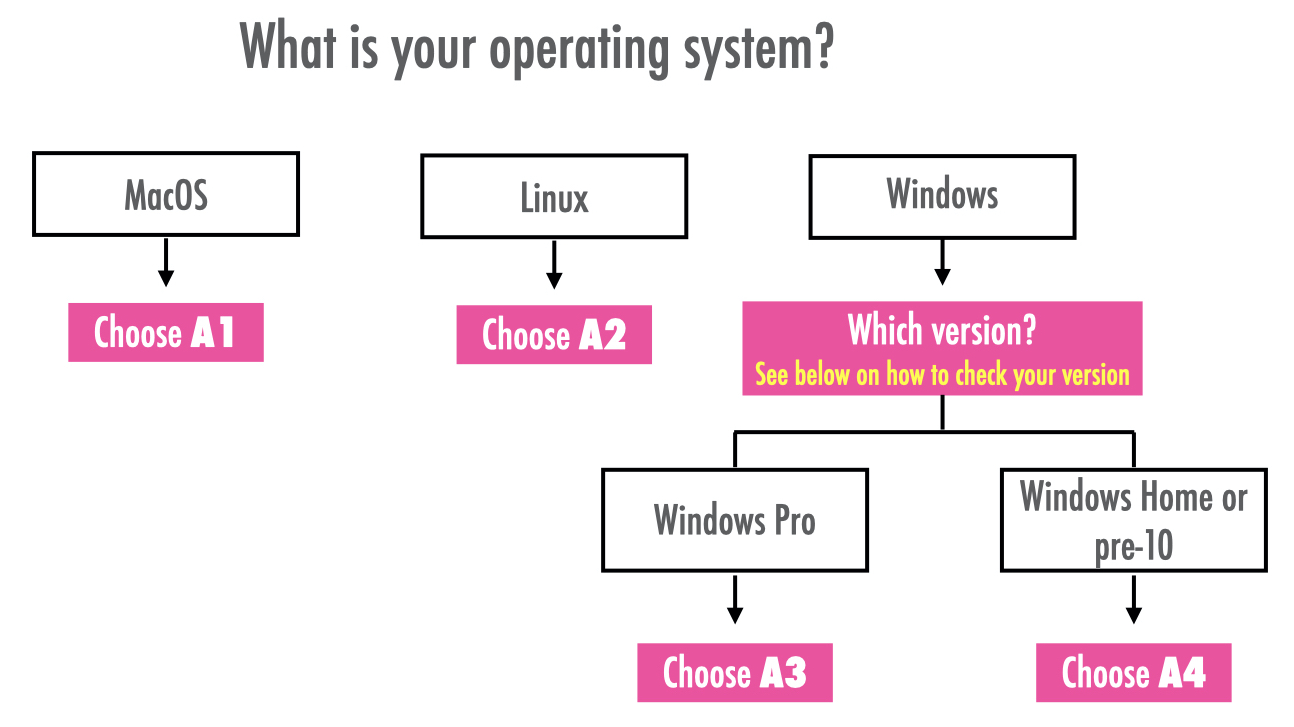
\includegraphics[width=17.97in]{figs/intro/tree} \end{center}

\textbf{A1} \href{mac.html}{MacOS Installation}

\textbf{A2} \href{linux.html}{Linux Installation}

\textbf{A3} \href{win10pro.html}{Windows 10 Pro/Student Installation}

\textbf{A4} \href{otherwin.html}{Windows Home or pre-10 Installation}

\emph{Need to find out your Windows version?} Click \href{version.html}{HERE}

\hypertarget{macos-installation}{%
\chapter*{MacOS Installation}\label{macos-installation}}
\addcontentsline{toc}{chapter}{MacOS Installation}

\hypertarget{installing-python}{%
\section*{Installing Python}\label{installing-python}}
\addcontentsline{toc}{section}{Installing Python}

\hypertarget{requirements}{%
\subsection*{Requirements}\label{requirements}}
\addcontentsline{toc}{subsection}{Requirements}

\begin{enumerate}
\def\labelenumi{\arabic{enumi}.}
\tightlist
\item
  A stable internet connection
\item
  \textasciitilde10GB of space on your hard drive
\item
  MacOS version 10.13 or newer i.e.~High Sierra, Mojave or Catalina. If you are unsure what version you are running click on the apple icon in the top left of the screen and then \textbf{About this Mac}.
\item
  Mac hardware must be a 2010 model or newer
\end{enumerate}

\hypertarget{installation-steps}{%
\subsection*{Installation steps}\label{installation-steps}}
\addcontentsline{toc}{subsection}{Installation steps}

\begin{enumerate}
\def\labelenumi{\arabic{enumi}.}
\tightlist
\item
  Go to the \href{https://hub.docker.com/editions/community/docker-ce-desktop-mac/}{dockerhub website}.
\item
  Ensure you meet the criteria for download (it is the same as stated above) and then select `Get Stable' button.
\end{enumerate}

\begin{center}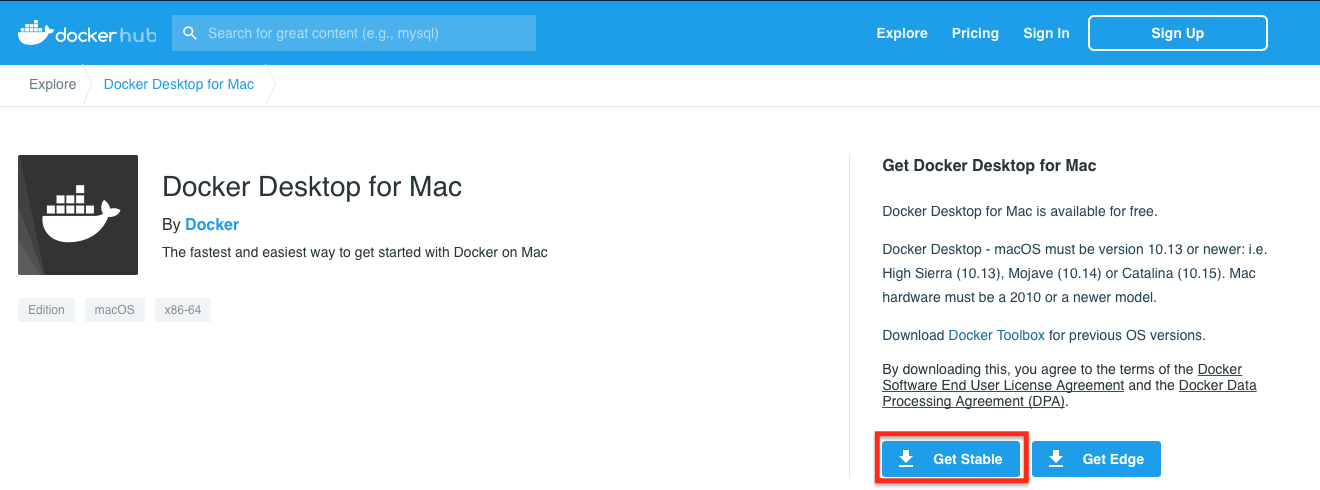
\includegraphics[width=18.33in]{figs/chp1/Figure1} \end{center}

\begin{enumerate}
\def\labelenumi{\arabic{enumi}.}
\setcounter{enumi}{2}
\tightlist
\item
  This will then download to your machine but may take some time. Once finished, to access this download go to \textbf{Finder} \textgreater{} \textbf{Downloads} \textgreater{} \textbf{Docker.dmg} and double click.
\end{enumerate}

\begin{center}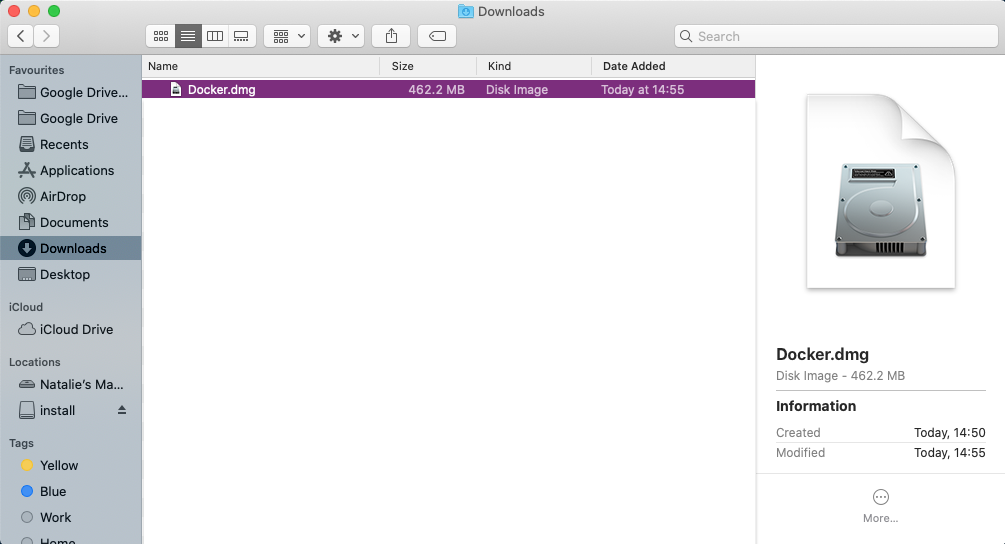
\includegraphics[width=13.96in]{figs/chp1/Figure2} \end{center}

\begin{enumerate}
\def\labelenumi{\arabic{enumi}.}
\setcounter{enumi}{3}
\tightlist
\item
  You should then be prompted to drag and drop this application into the applications folder like so:
\end{enumerate}

\begin{center}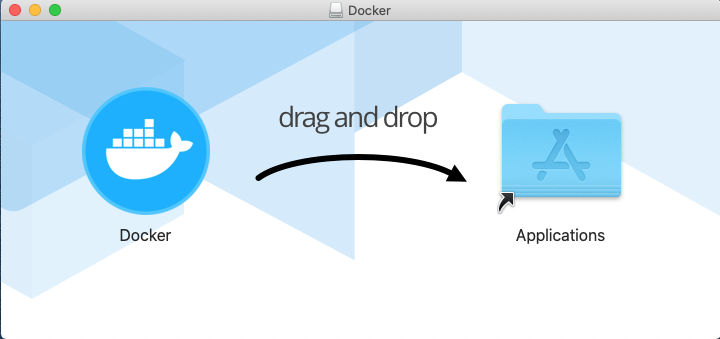
\includegraphics[width=10in]{figs/chp1/Figure3} \end{center}

You may get further windows asking for access to the program. To these you can click \textbf{Open} \textgreater{} \textbf{Ok} \textgreater{} enter your account password and click \textbf{Install helper}

\begin{enumerate}
\def\labelenumi{\arabic{enumi}.}
\setcounter{enumi}{4}
\tightlist
\item
  After you have done this, the whale icon should now show in your taskbar:
\end{enumerate}

\begin{center}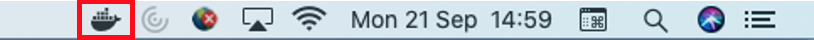
\includegraphics[width=11.31in]{figs/chp1/Figure4} \end{center}

You have successfully downloaded Docker!

Next steps: \protect\hyperlink{using-docker}{Using Docker}

\hypertarget{using-docker}{%
\subsection*{Using Docker}\label{using-docker}}
\addcontentsline{toc}{subsection}{Using Docker}

Now we have Docker installed we can use it to access Python and all the associated packages we need for the practicals

\hypertarget{installing-the-gds-environment}{%
\subsection*{Installing the GDS environment}\label{installing-the-gds-environment}}
\addcontentsline{toc}{subsection}{Installing the GDS environment}

\begin{enumerate}
\def\labelenumi{\arabic{enumi}.}
\tightlist
\item
  Access your terminal: \textbf{Launchpad} \textgreater{} \textbf{Other} \textgreater{} \textbf{Terminal}
\item
  In a fresh line in the terminal type the following to install the GDS environment container: \texttt{docker\ pull\ darribas/gds:5.0}
\end{enumerate}

\begin{center}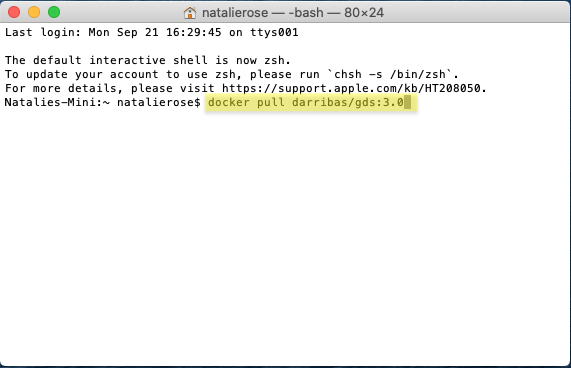
\includegraphics[width=7.94in]{figs/chp1/Figure5} \end{center}

\begin{enumerate}
\def\labelenumi{\arabic{enumi}.}
\setcounter{enumi}{2}
\tightlist
\item
  This should now prompt a long download process that looks a bit like this:
\end{enumerate}

\begin{center}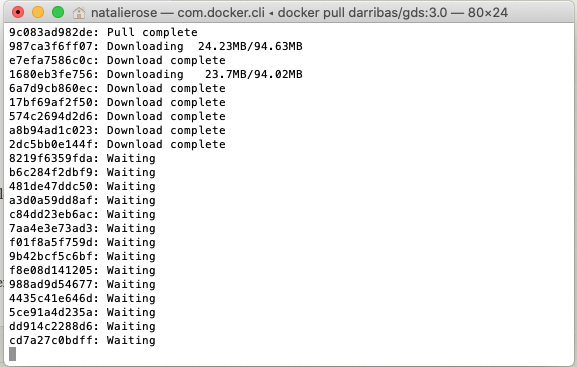
\includegraphics[width=7.94in]{figs/chp1/Figure6} \end{center}

Dont be alarmed if it seems to take a very long time.

You will know this has completed when each line says `Pull complete' and the new line gives your machine name followed by a \texttt{\$} sign.

\hypertarget{running-python}{%
\section*{Running Python}\label{running-python}}
\addcontentsline{toc}{section}{Running Python}

\hypertarget{running-the-container}{%
\subsection*{Running the container}\label{running-the-container}}
\addcontentsline{toc}{subsection}{Running the container}

\begin{enumerate}
\def\labelenumi{\arabic{enumi}.}
\tightlist
\item
  In the new terminal line type the following command to run the container: \texttt{docker\ run\ -\/-rm\ -ti\ -p\ 8888:8888\ -v\ \$\{PWD\}:/home/jovyan/work\ darribas/gds:5.0}
\end{enumerate}

\begin{center}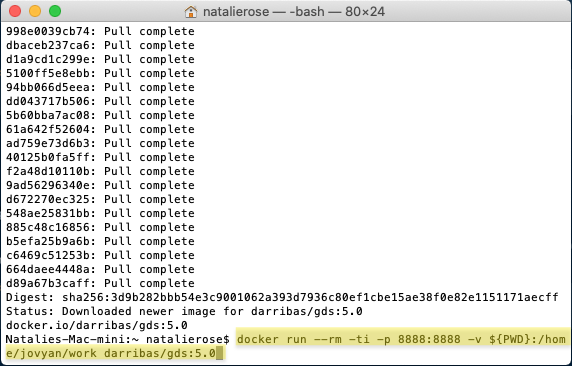
\includegraphics[width=7.94in]{figs/chp1/Figure7} \end{center}

You have now started a Python session.

\textbf{NOTE: It is important that you do not close the terminal window until you are finished in this Python session}

\begin{enumerate}
\def\labelenumi{\arabic{enumi}.}
\setcounter{enumi}{1}
\item
  To access this session go to your chosen web browser (e.g.~Safari/Chrome) and type: \texttt{localhost:8888} into the search bar
\item
  The page that loads will prompt you for a password. This password can be found in the text in the terminal following the last command you ran (step 9). A long series of numbers and letters will be preceded by \texttt{?token=}. Copy this long series of characters and paste into the password box in your browser.
\end{enumerate}

\begin{center}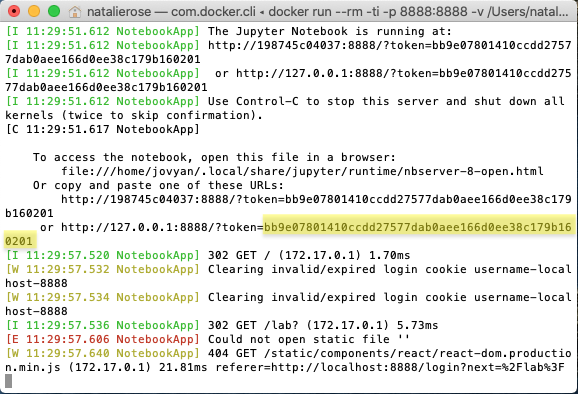
\includegraphics[width=7.94in]{figs/chp1/Figure9} \end{center}

\begin{center}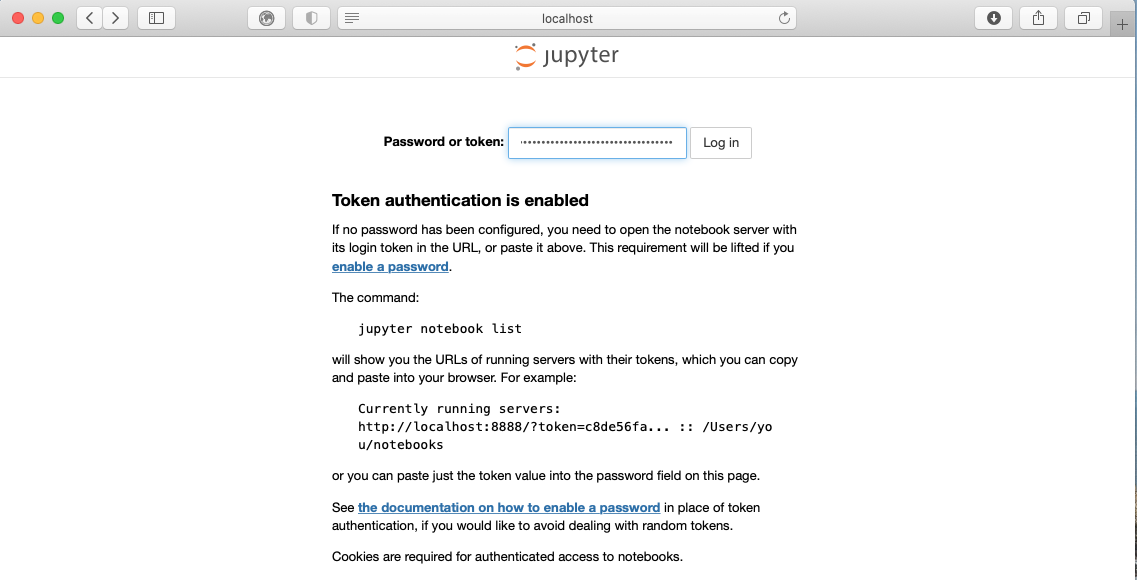
\includegraphics[width=15.79in]{figs/chp1/Figure10} \end{center}

\begin{enumerate}
\def\labelenumi{\arabic{enumi}.}
\setcounter{enumi}{3}
\tightlist
\item
  Now you are in Jupyter Lab you can open up a Python 3 notebook
\end{enumerate}

\begin{center}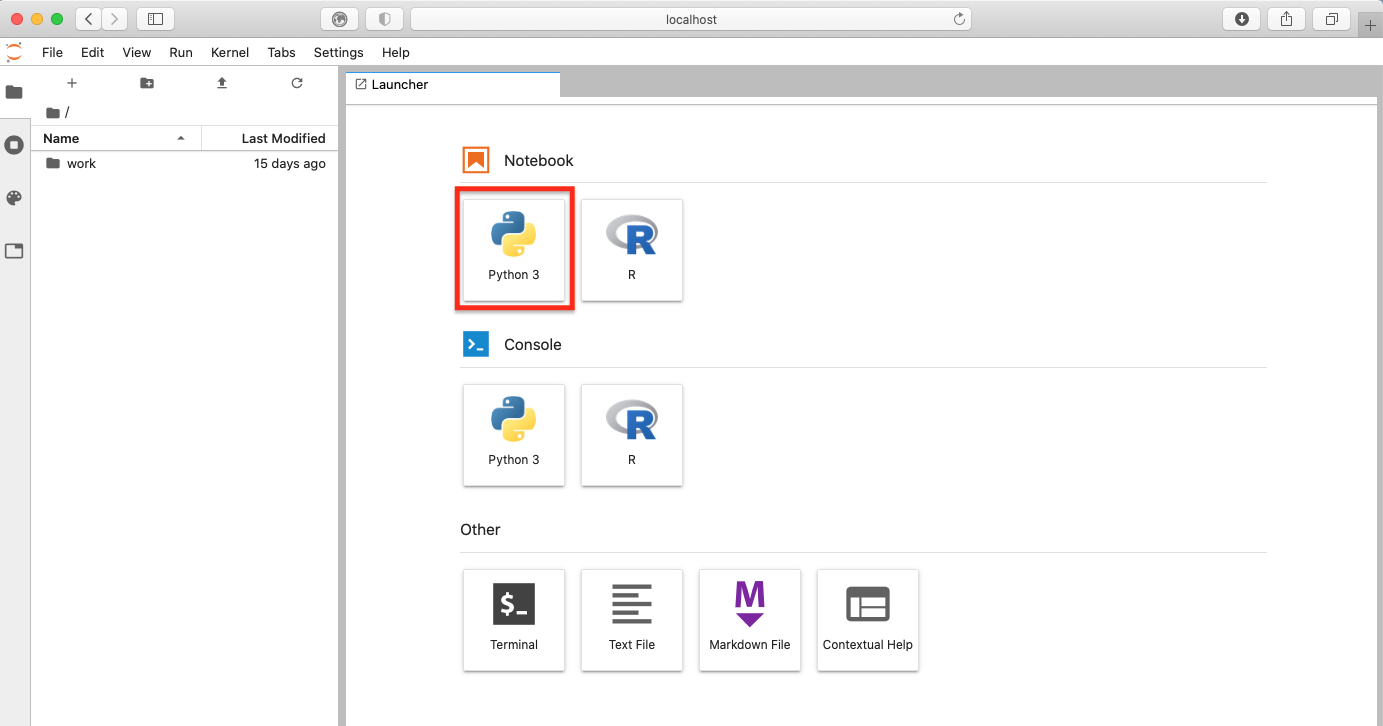
\includegraphics[width=19.21in]{figs/chp1/Figure11} \end{center}

\protect\hyperlink{using-jupyter-notebook}{Using Jupyter Notebook}

\hypertarget{using-jupyter-notebook}{%
\subsection*{Using Jupyter Notebook}\label{using-jupyter-notebook}}
\addcontentsline{toc}{subsection}{Using Jupyter Notebook}

\begin{itemize}
\tightlist
\item
  This notebook is where you will run your code. Each shaded box is called a kernel. To test this out you can type \texttt{print(\textquotesingle{}test\textquotesingle{})} into one of these kernels. To run the code use the shortcut \texttt{Ctrl\ +\ Enter}.
\end{itemize}

\begin{center}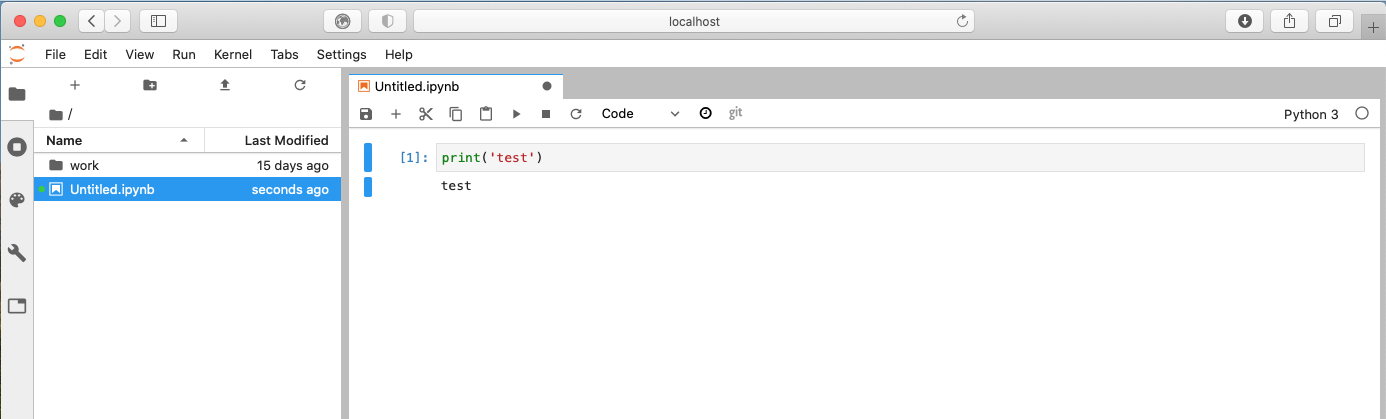
\includegraphics[width=19.25in]{figs/chp1/Figure12} \end{center}

\begin{itemize}
\tightlist
\item
  You can save your notebook using \textbf{File} \textgreater{} \textbf{Save notebook as}
\end{itemize}

\begin{center}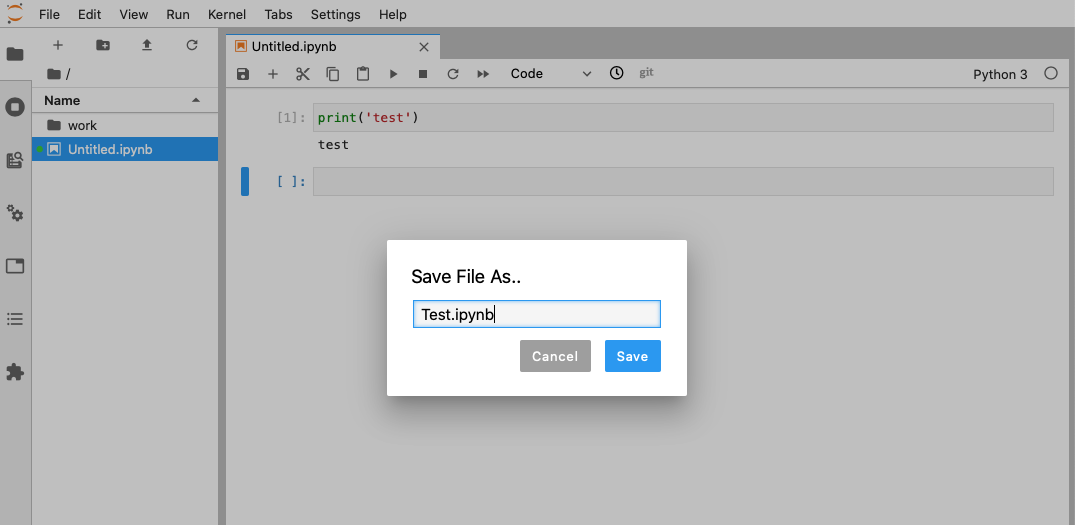
\includegraphics[width=14.93in]{figs/chp1/Figure13} \end{center}

\begin{itemize}
\tightlist
\item
  You can create new folders to organise your work
\end{itemize}

\begin{center}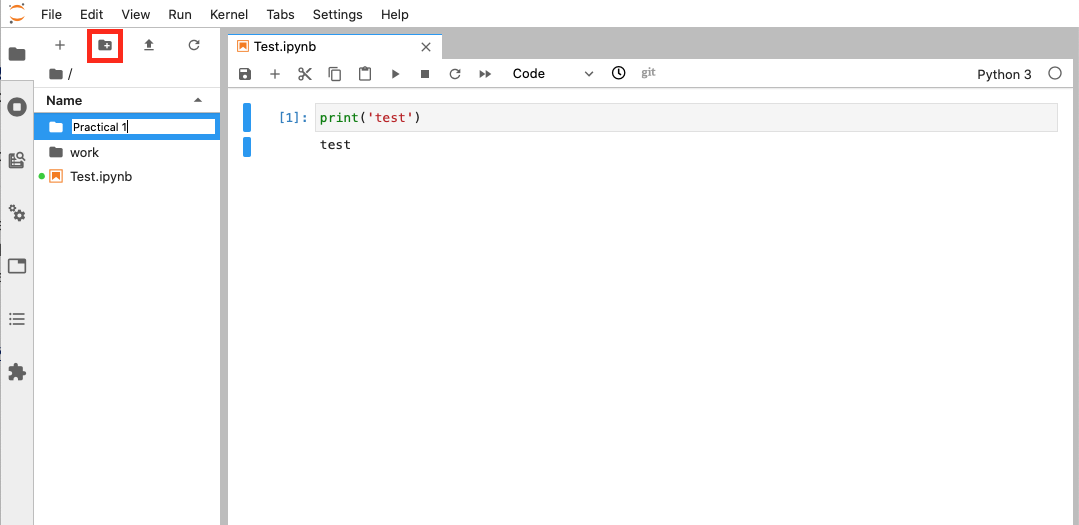
\includegraphics[width=14.99in]{figs/chp1/Figure14} \end{center}

\begin{itemize}
\tightlist
\item
  And you can access other files on your machine through the `Work' folder in the File Browser. From here you can navigate to your Documents and designated folder for this module
\end{itemize}

\begin{center}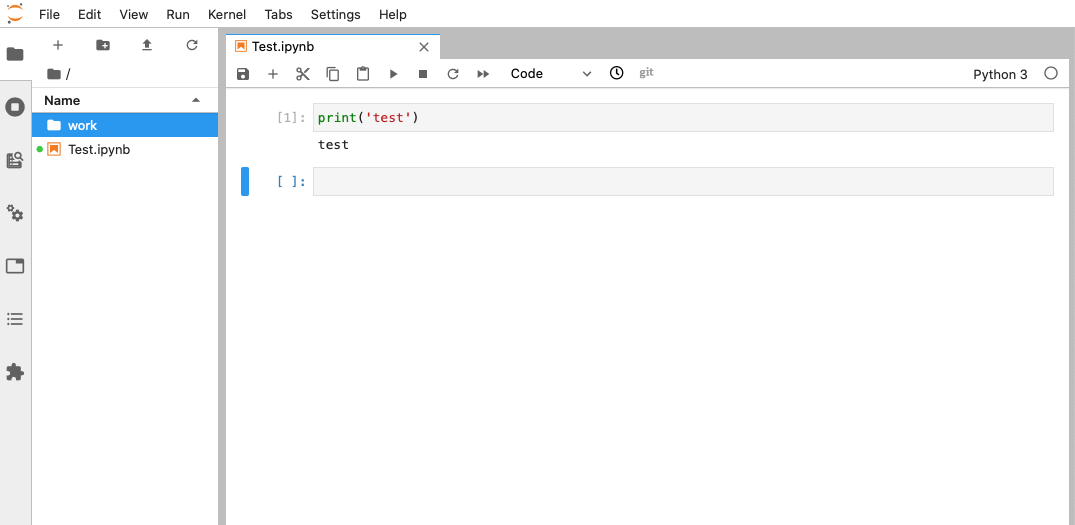
\includegraphics[width=14.93in]{figs/chp1/Figure15a} \end{center}

\begin{center}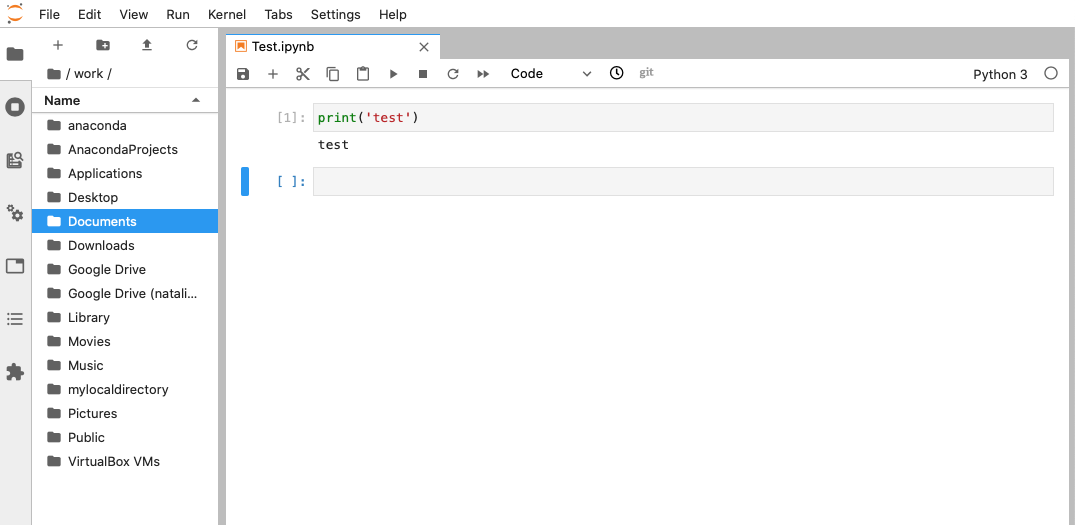
\includegraphics[width=14.93in]{figs/chp1/Figure15b} \end{center}

\begin{center}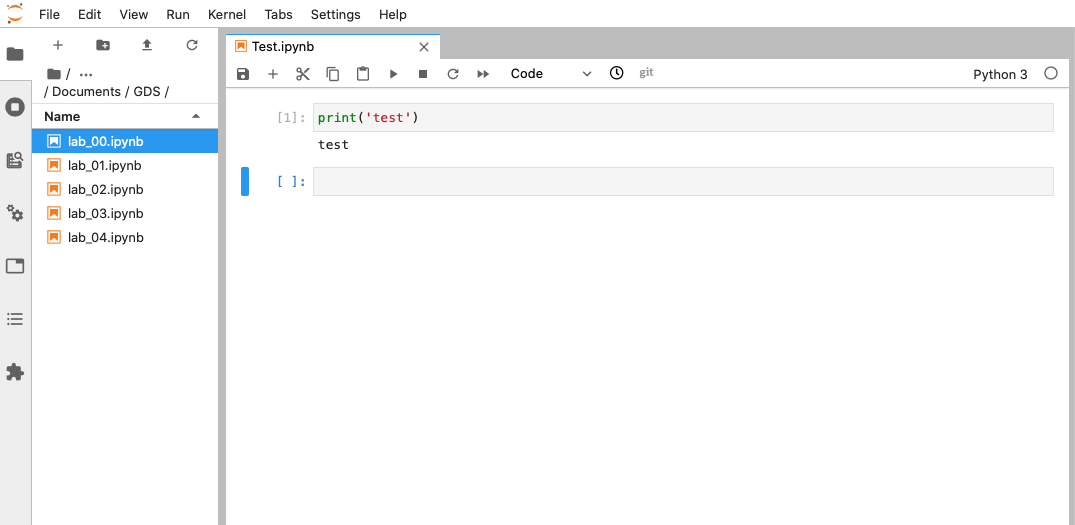
\includegraphics[width=14.93in]{figs/chp1/Figure15c} \end{center}

\protect\hyperlink{ending-your-session}{Ending your session}

\hypertarget{ending-your-session}{%
\subsection*{Ending your session}\label{ending-your-session}}
\addcontentsline{toc}{subsection}{Ending your session}

Once you have finished in your Jupyter session and have saved all your work, you can end the session from the terminal.

Using \texttt{Ctrl\ +\ C} will prompt a \texttt{y/n} option. Either type \texttt{y} or \texttt{Ctrl\ +\ C} again to end the session.

\begin{center}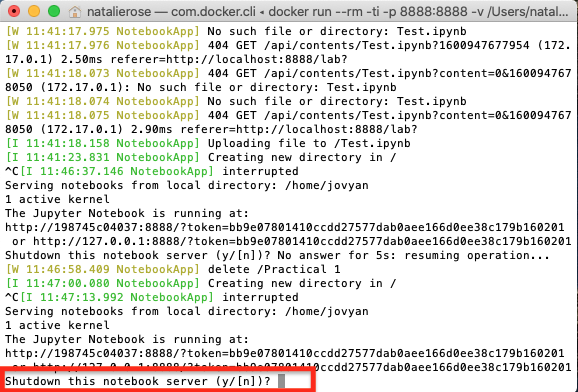
\includegraphics[width=8.03in]{figs/chp1/Figure16} \end{center}

You can now safely shut the terminal window.

Next time you go to run a Jupyter Notebook you will not need to repeat the whole process as you have already installed Docker and the GDS environment. Instead you can start from \protect\hyperlink{running-the-container}{Running the container} and carry on from there.

\hypertarget{linux-installation}{%
\chapter*{Linux Installation}\label{linux-installation}}
\addcontentsline{toc}{chapter}{Linux Installation}

Instructions to install, test and run \texttt{gds\_env} with Docker for .

For each of the sections, add:

\begin{quote}
Step-by-step instructions
\end{quote}

\begin{quote}
Insert screenshots for each step
\end{quote}

\begin{quote}
Insert a video with instructions
\end{quote}

\hypertarget{installing-docker}{%
\section*{Installing Docker}\label{installing-docker}}
\addcontentsline{toc}{section}{Installing Docker}

Draw on instructions from \href{https://gdsl-ul.github.io/the_knowledge/docker.html}{here} and \href{https://darribas.org/gds_env/guides/docker_install/}{here} and \href{https://darribas.org/gds_env/guides/docker_install/}{here}

\hypertarget{requirements}{%
\subsection*{Requirements}\label{requirements}}
\addcontentsline{toc}{subsection}{Requirements}

\hypertarget{install-steps}{%
\subsection*{Install steps}\label{install-steps}}
\addcontentsline{toc}{subsection}{Install steps}

\hypertarget{check-success}{%
\subsection*{Check success}\label{check-success}}
\addcontentsline{toc}{subsection}{Check success}

\hypertarget{running-python-through-docker}{%
\section*{Running Python through Docker}\label{running-python-through-docker}}
\addcontentsline{toc}{section}{Running Python through Docker}

\hypertarget{windows-10-prostudent-installation}{%
\chapter*{Windows 10 Pro/Student Installation}\label{windows-10-prostudent-installation}}
\addcontentsline{toc}{chapter}{Windows 10 Pro/Student Installation}

\hypertarget{windows-home-or-pre-10-installation}{%
\chapter*{Windows Home or pre-10 Installation}\label{windows-home-or-pre-10-installation}}
\addcontentsline{toc}{chapter}{Windows Home or pre-10 Installation}

\hypertarget{installing-python}{%
\section*{Installing Python}\label{installing-python}}
\addcontentsline{toc}{section}{Installing Python}

\hypertarget{environment-file}{%
\subsection*{Environment File}\label{environment-file}}
\addcontentsline{toc}{subsection}{Environment File}

We will start by downloading an environment file, which will later on install all packages that are relevant for your coding

\textbf{NOTE: It would be best to create a dedicated folder (e.g.~GDS\_2020) for this module.}

\begin{center}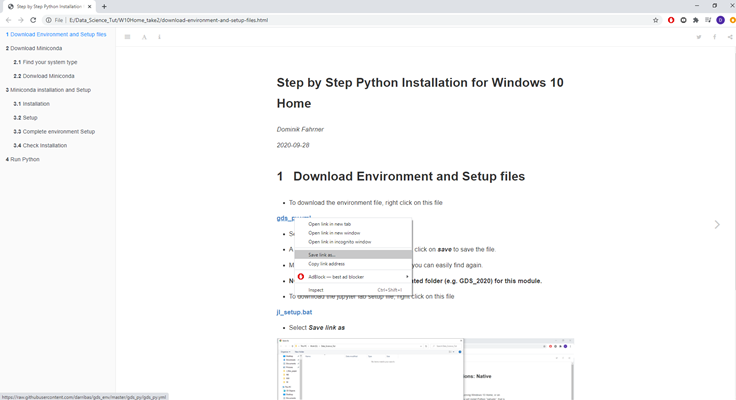
\includegraphics[width=10.22in]{figs/chp4/Picture4} \end{center}

\begin{itemize}
\tightlist
\item
  To download the environment file, right click on this file
\end{itemize}

\href{https://raw.githubusercontent.com/darribas/gds_env/master/gds_py/gds_py.yml}{\textbf{gds\_py.yml}}

\begin{itemize}
\tightlist
\item
  Select \textbf{\emph{Save link as}}.
\end{itemize}

\begin{center}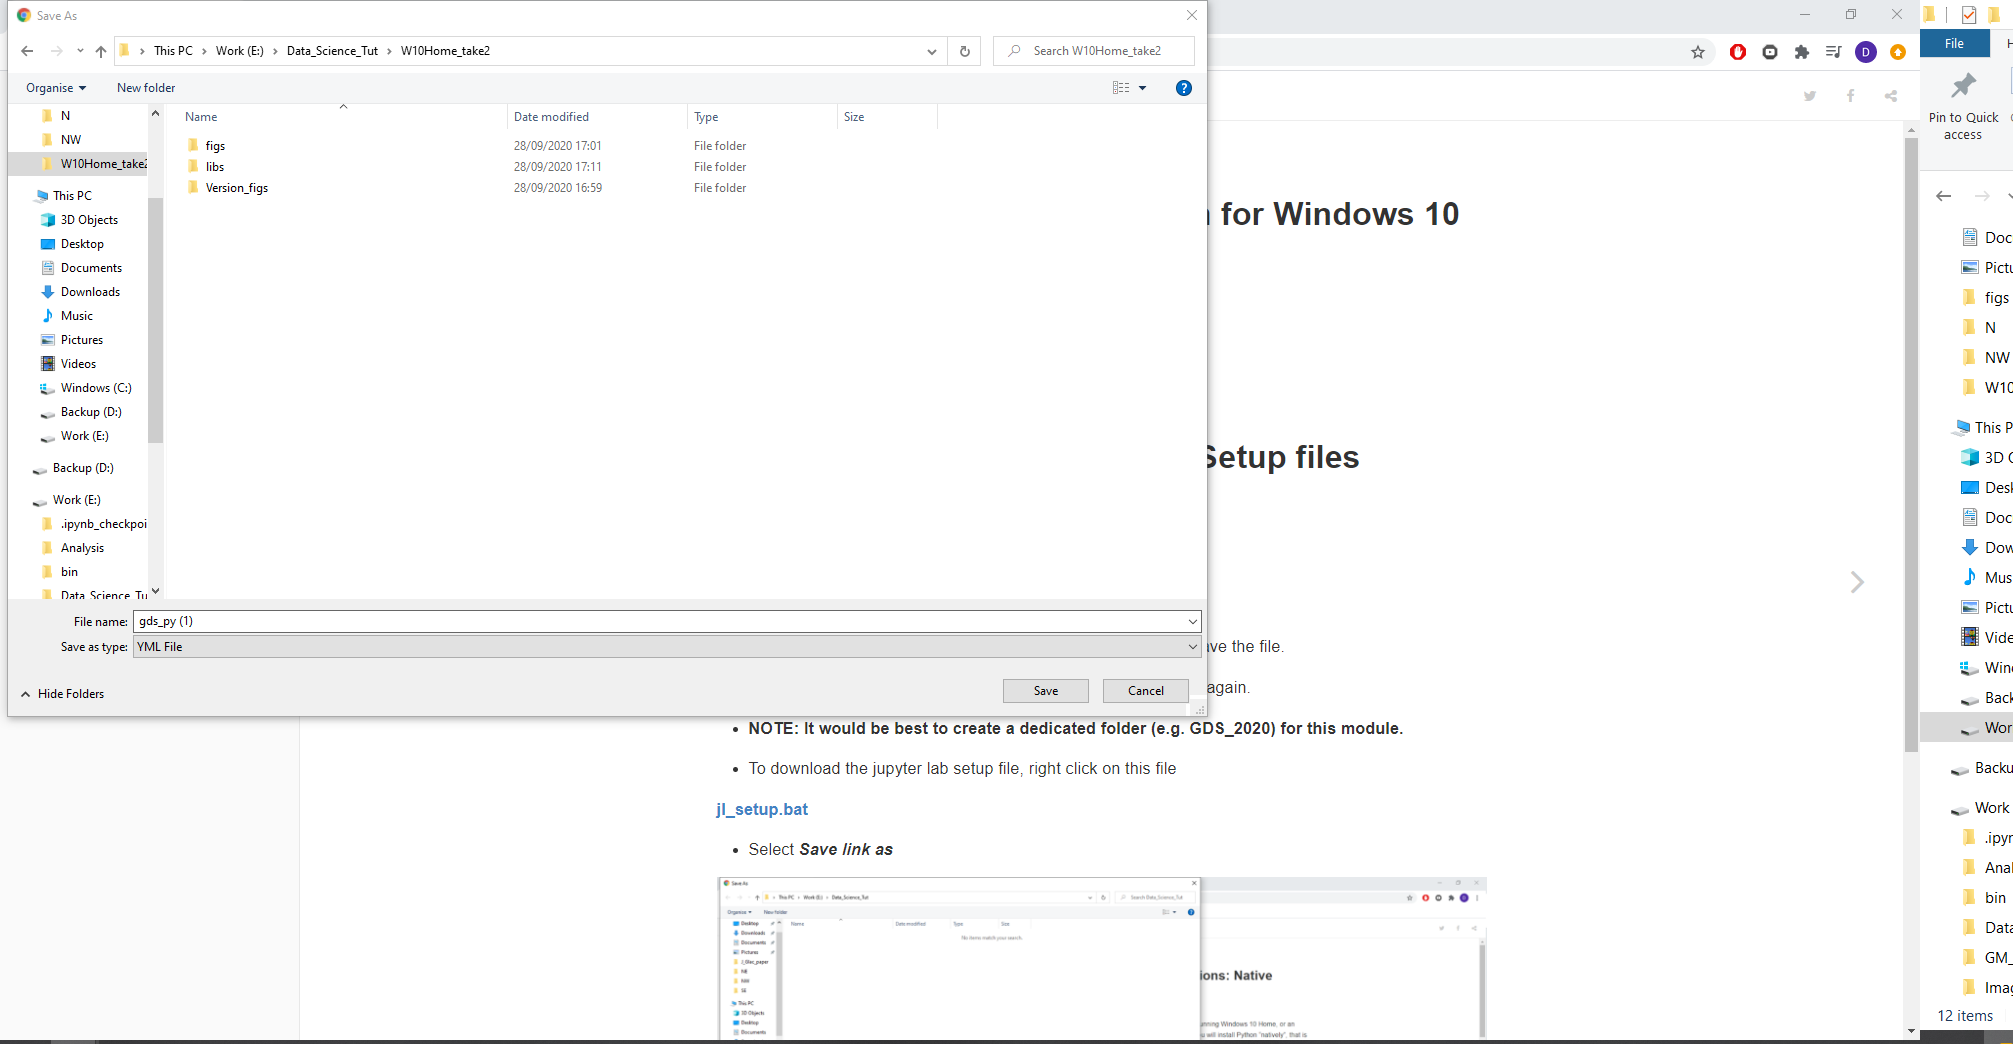
\includegraphics[width=27.96in]{figs/chp4/Picture5} \end{center}

\begin{itemize}
\tightlist
\item
  A new window will pop up for saving the file, click on \textbf{\emph{save}} to save the file.
\item
  Make sure to save the file to a location that you can easily find again.
\end{itemize}

\hypertarget{user-interface}{%
\subsection*{User interface}\label{user-interface}}
\addcontentsline{toc}{subsection}{User interface}

We will now download the file that will later setup your coding interface (which is called Jupyter Lab).

\begin{itemize}
\tightlist
\item
  To download the jupyter lab setup file, right click on this file
\end{itemize}

\href{https://gdsl-ul.github.io/soft_install/jl_setup.bat}{\textbf{jl\_setup.bat}}

\begin{center}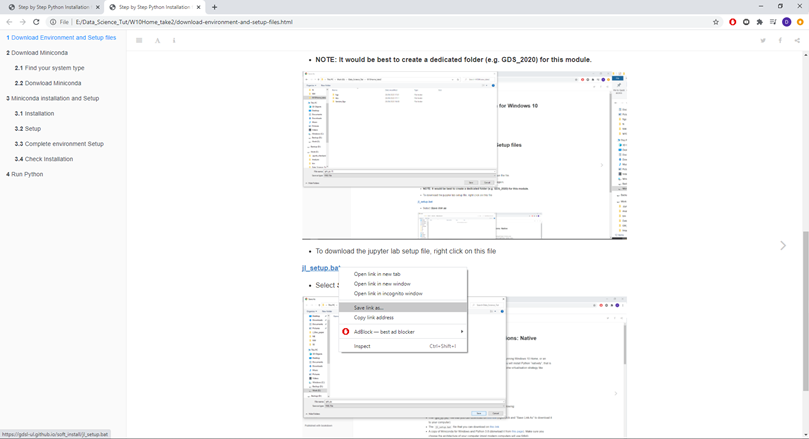
\includegraphics[width=11.24in]{figs/chp4/Picture6} \end{center}

\begin{itemize}
\tightlist
\item
  Select \textbf{\emph{Save link as}}
\end{itemize}

\begin{center}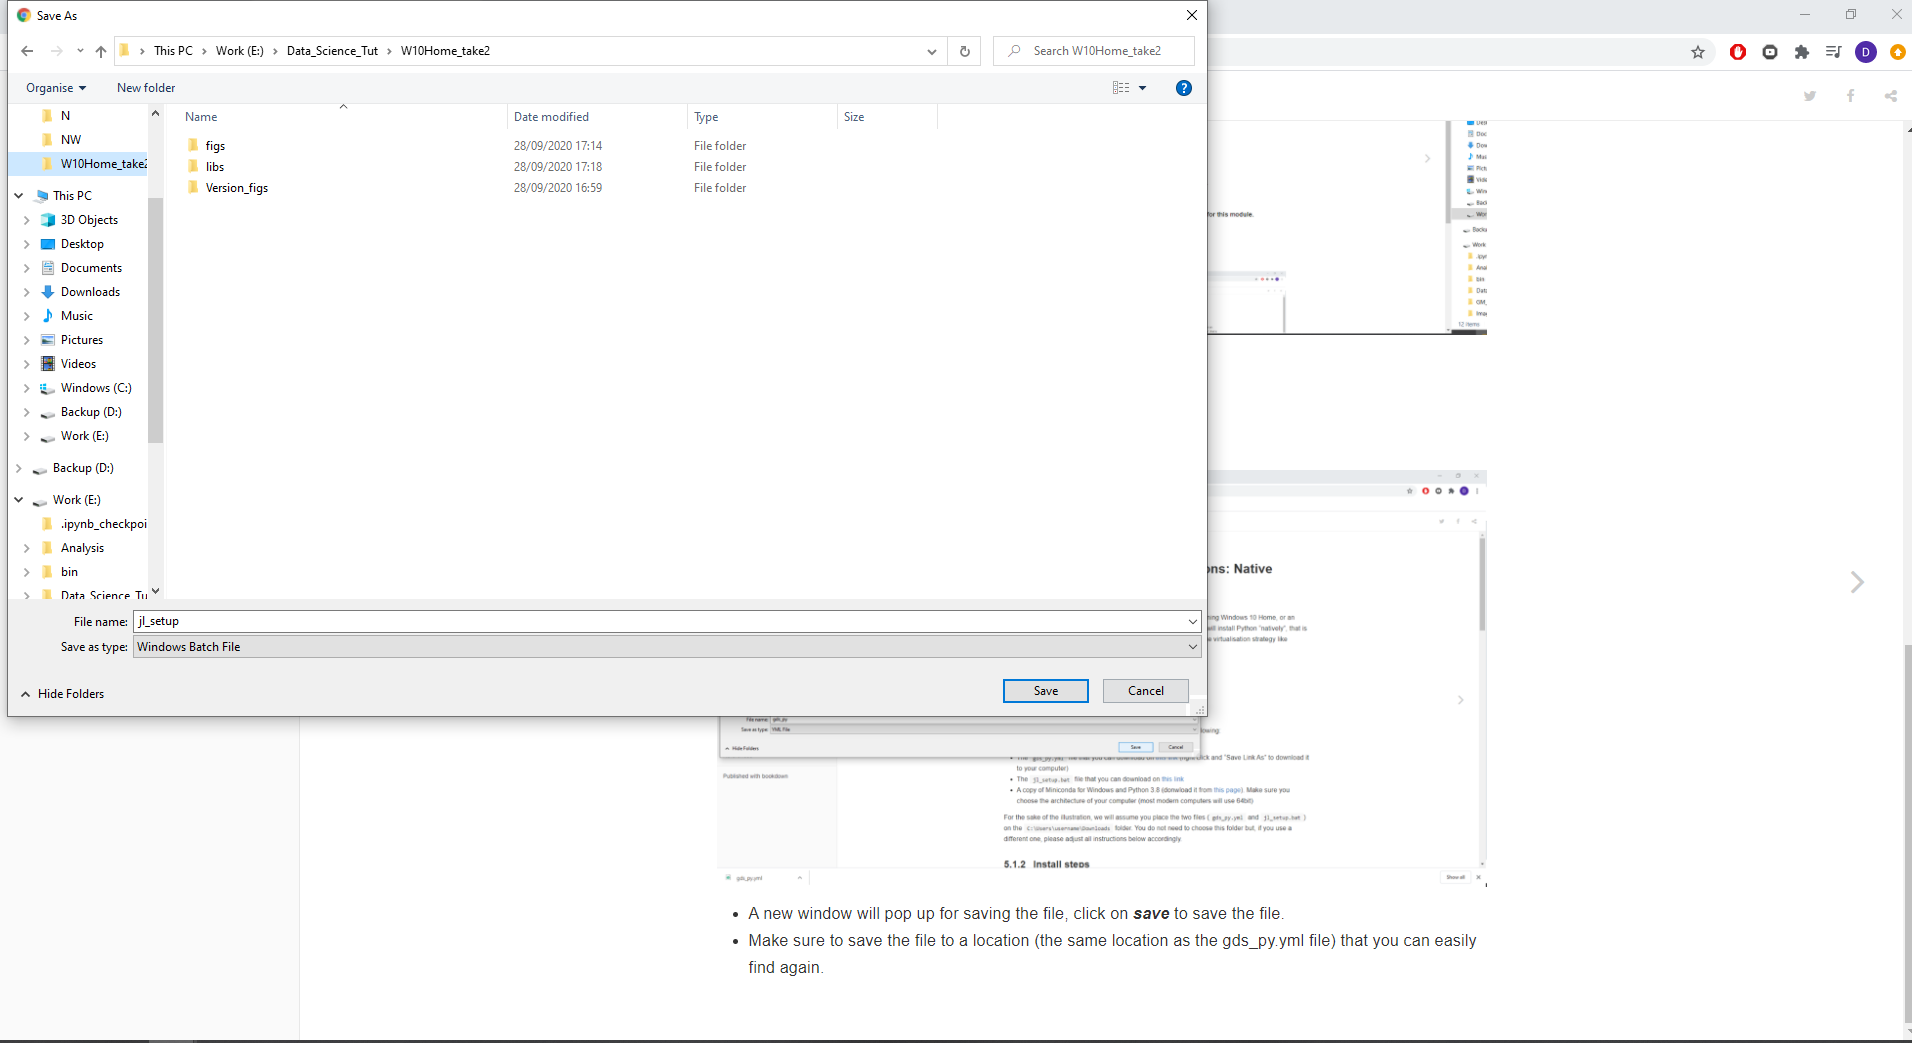
\includegraphics[width=26.56in]{figs/chp4/Picture6_1} \end{center}

\begin{itemize}
\tightlist
\item
  A new window will pop up for saving the file, click on \textbf{\emph{save}} to save the file.
\item
  Make sure to save the file to a location (the same location as the \texttt{gds\_py.yml} file) that you can easily find again.
\end{itemize}

\hypertarget{download-miniconda}{%
\subsection*{Download Miniconda}\label{download-miniconda}}
\addcontentsline{toc}{subsection}{Download Miniconda}

\begin{quote}
Find your system type
\end{quote}

Before you can download Miniconda (which is a version of Anaconda), you need to find out what type your Windows system is.
It can either be 32 bit or 64 bit (most modern computers use 64 bit).

\begin{center}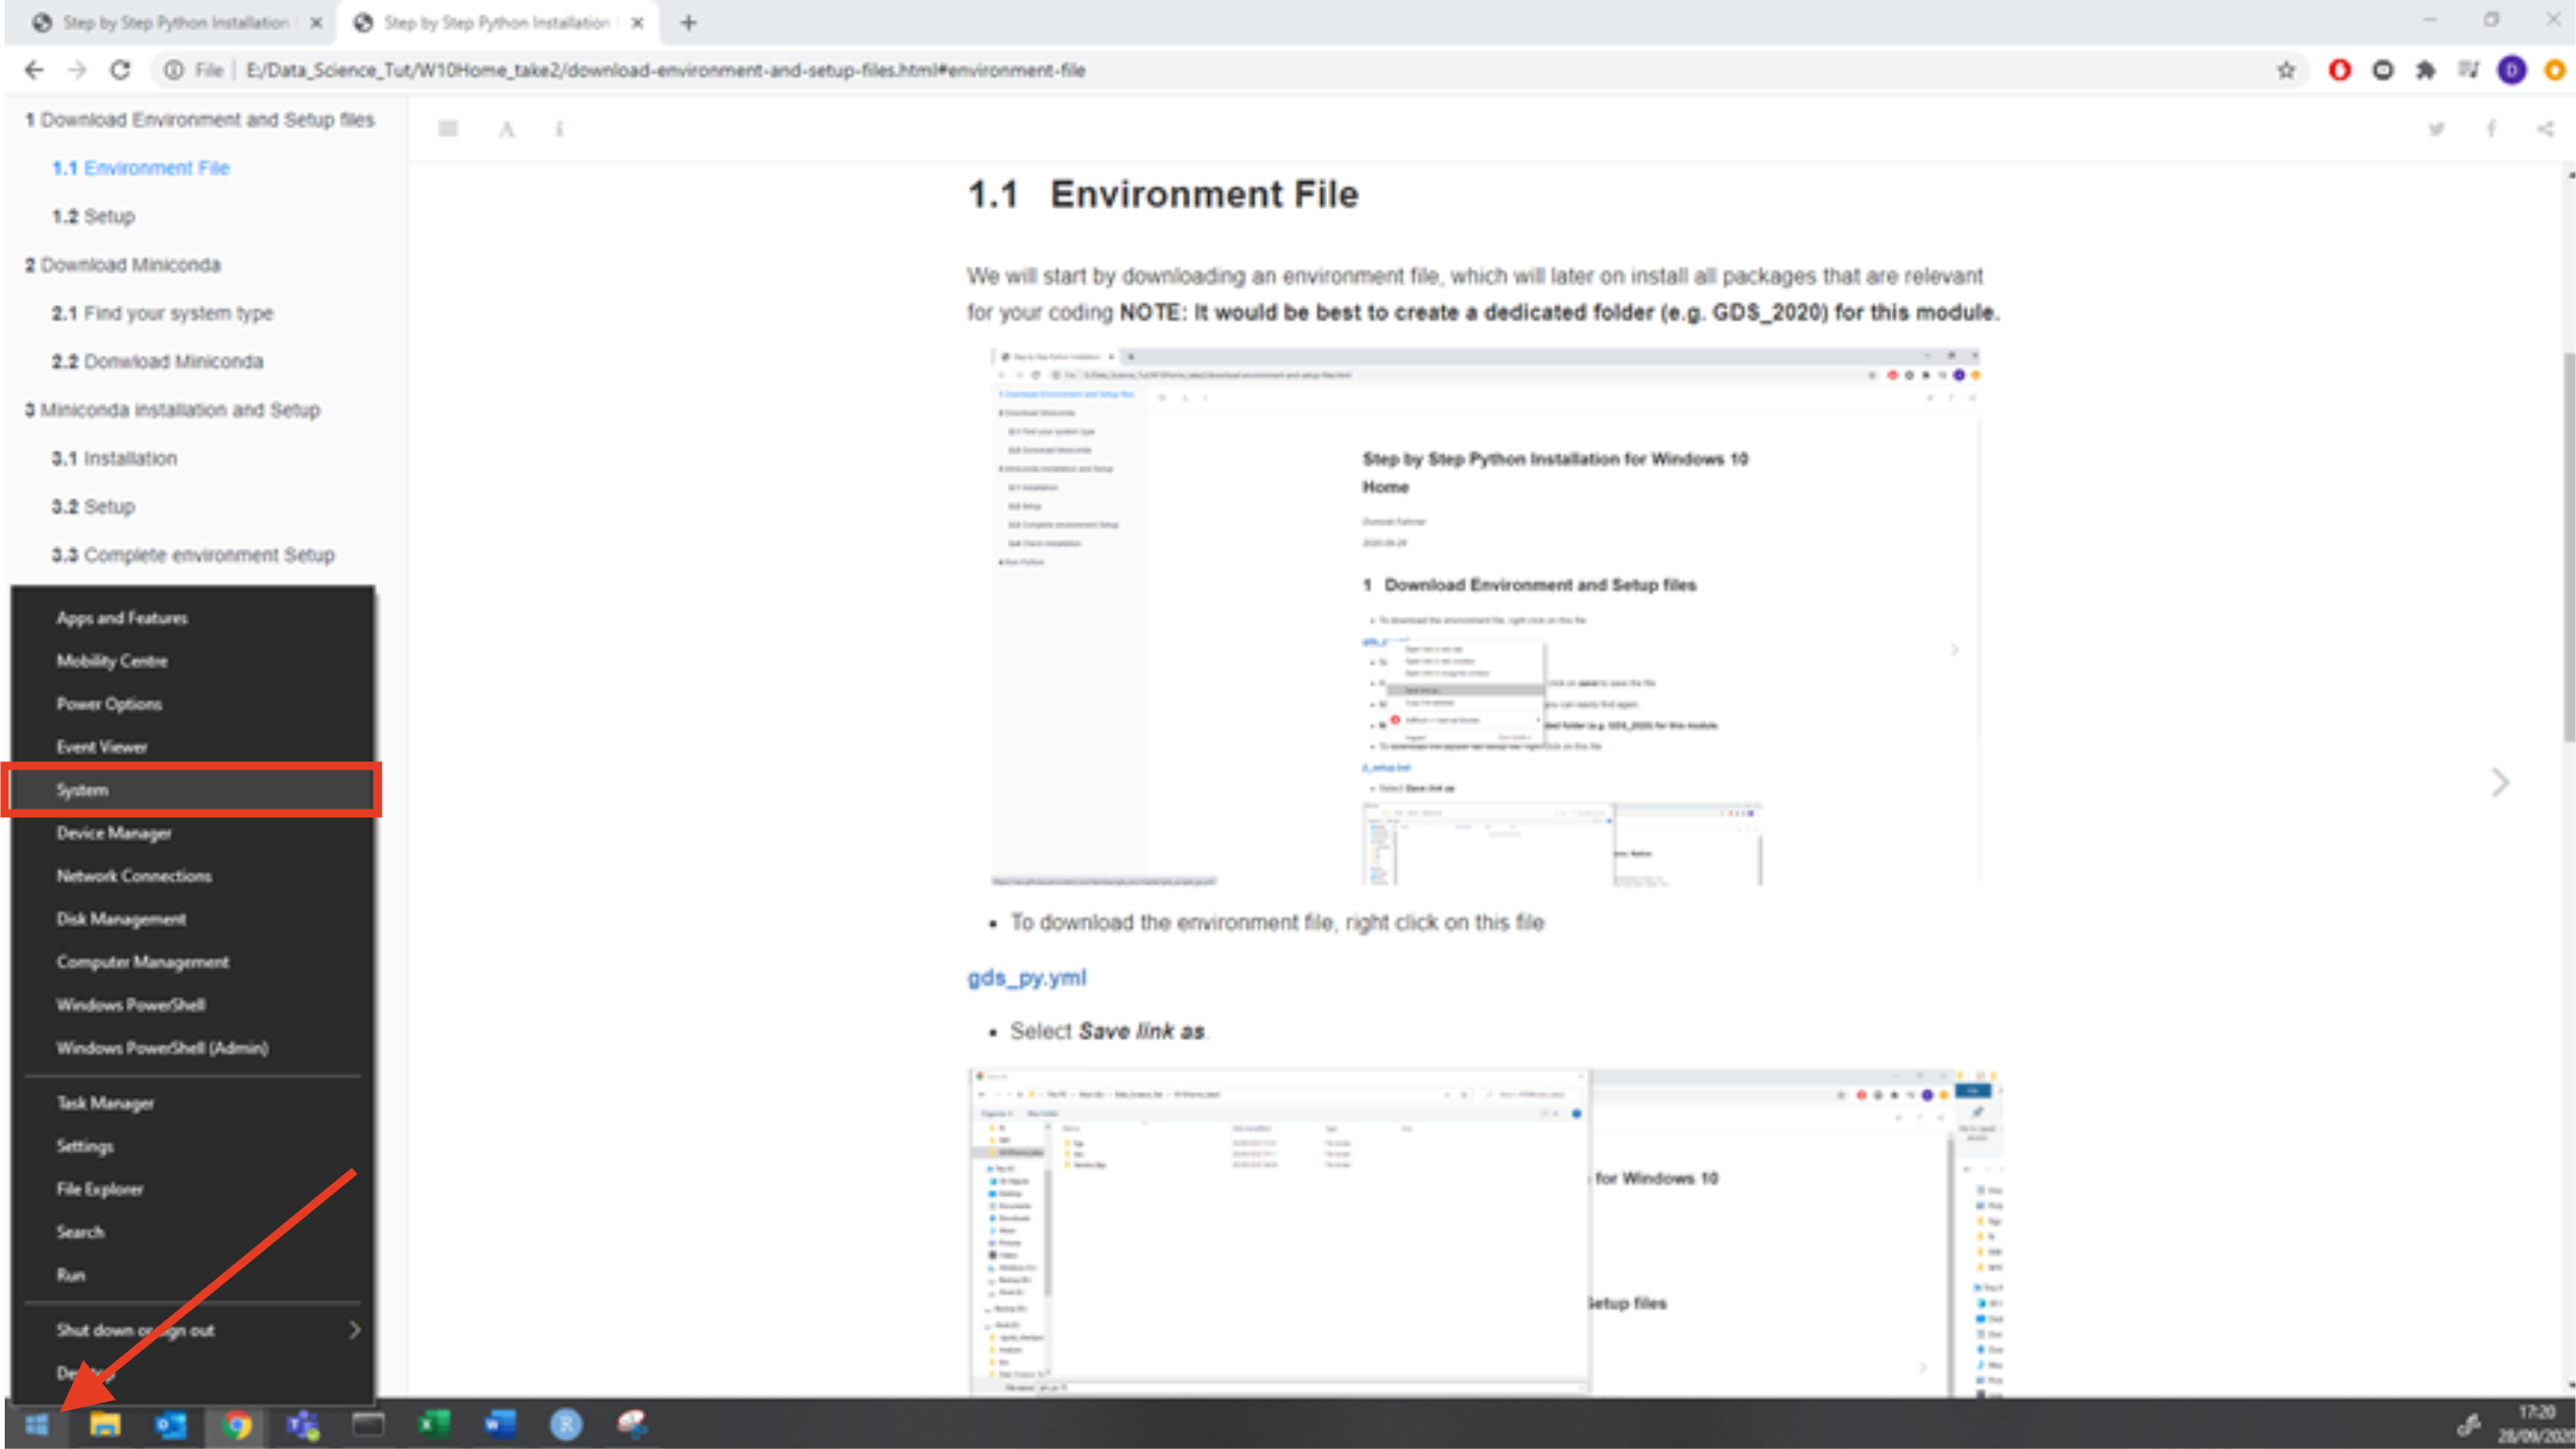
\includegraphics[width=37.67in]{figs/chp4/Picture7} \end{center}

\begin{itemize}
\tightlist
\item
  Right click on the windows logo in the left bottom corner of the task menu and select \textbf{System}
\end{itemize}

\begin{center}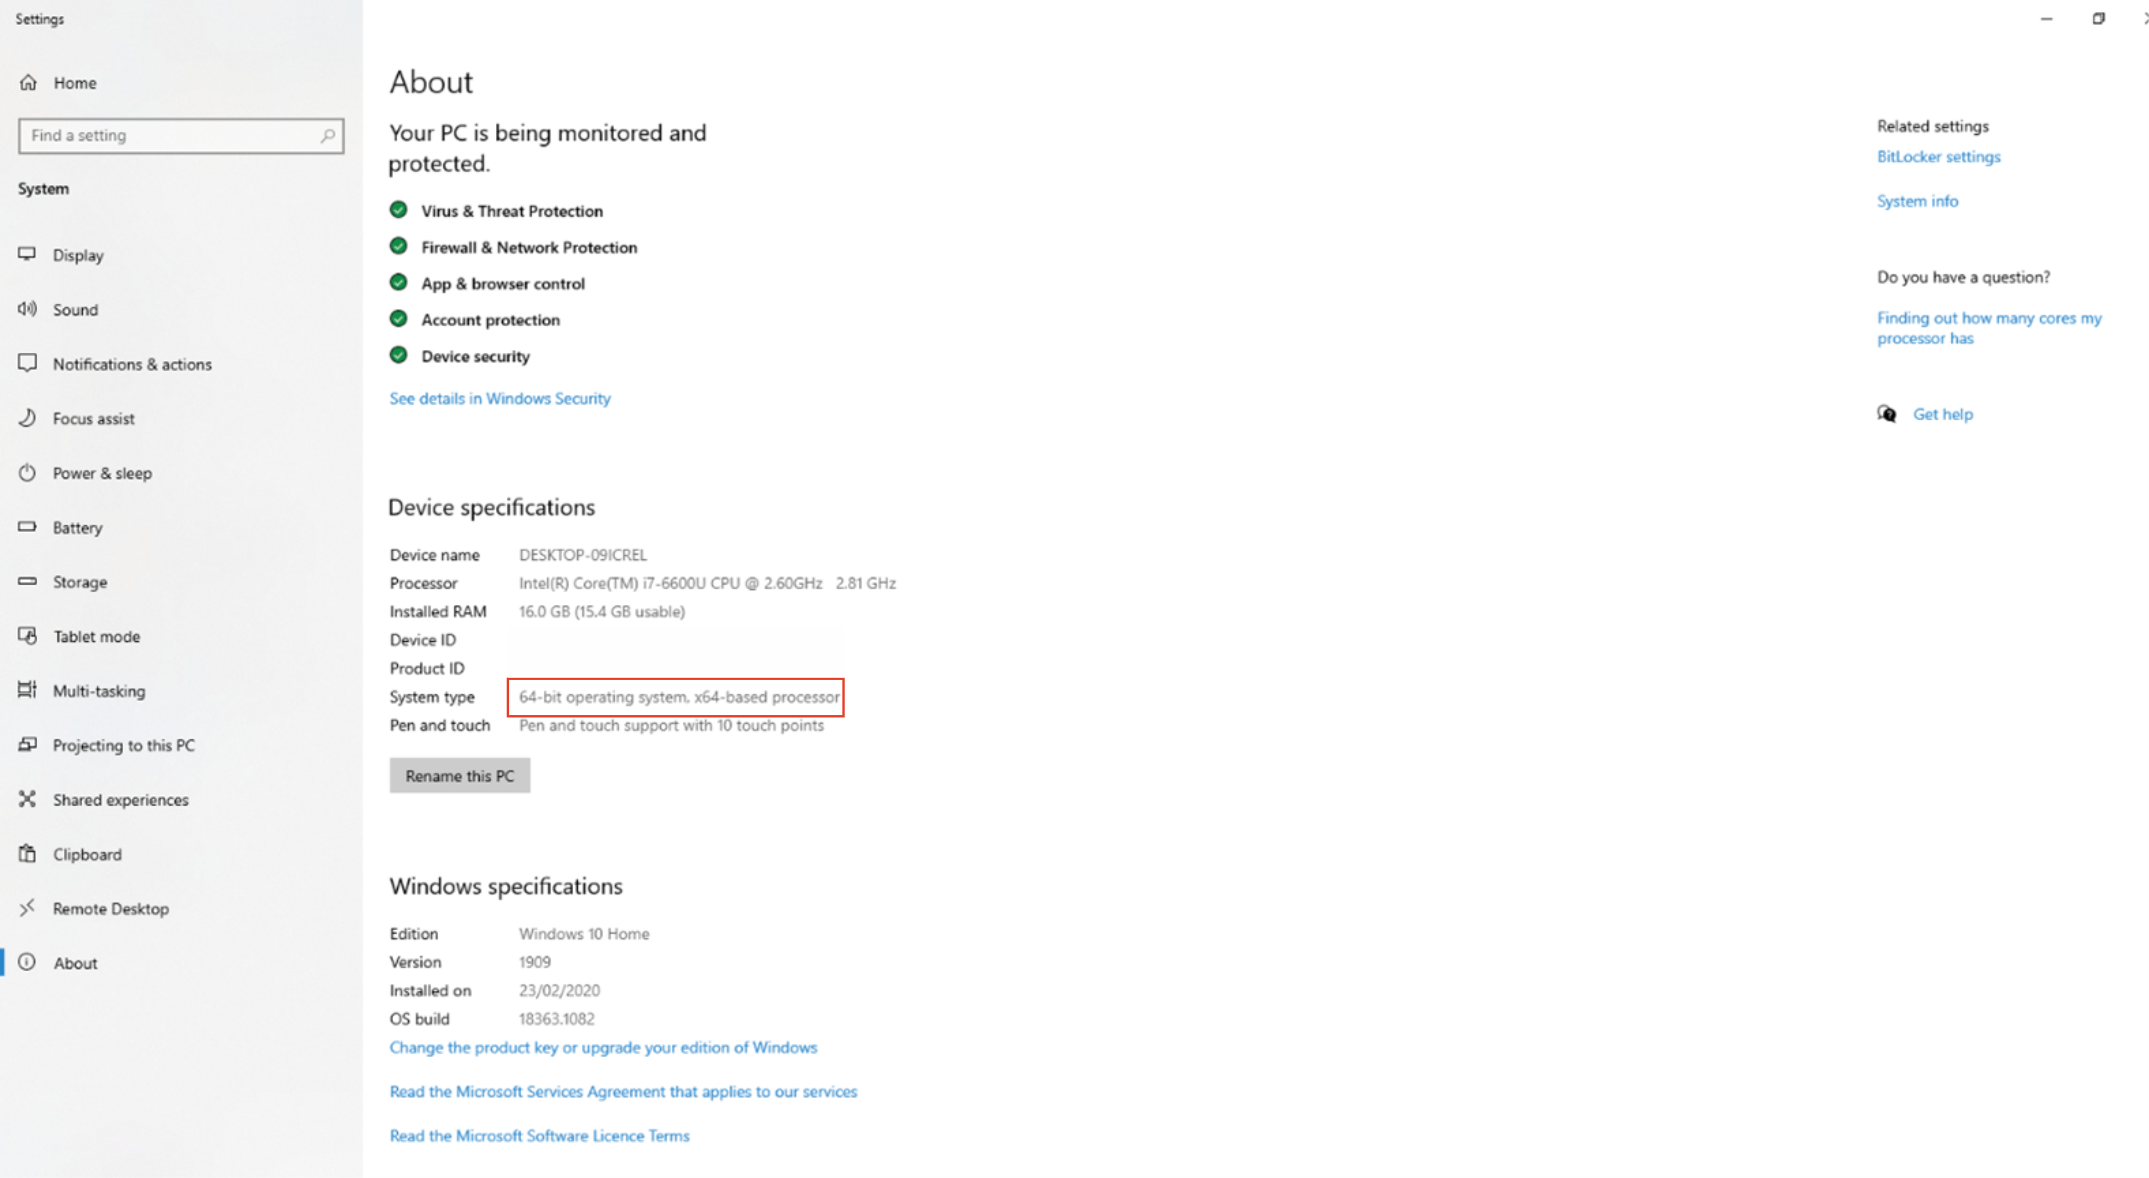
\includegraphics[width=29.85in]{figs/chp4/Picture8} \end{center}

\begin{itemize}
\tightlist
\item
  This will bring you to your system information page.
\item
  Look at the \textbf{System type} section and check if your operating system is 64-bit or 32-bit (highlighted in red).
\end{itemize}

\hypertarget{donwload-miniconda}{%
\subsection*{Donwload Miniconda}\label{donwload-miniconda}}
\addcontentsline{toc}{subsection}{Donwload Miniconda}

\begin{itemize}
\tightlist
\item
  Continue with opening this link to \href{https://docs.conda.io/en/latest/miniconda.html\#windows-installers}{\textbf{Miniconda}} by right clicking on the link and then selecting \textbf{\emph{Open in new tab}}.
\end{itemize}

\begin{center}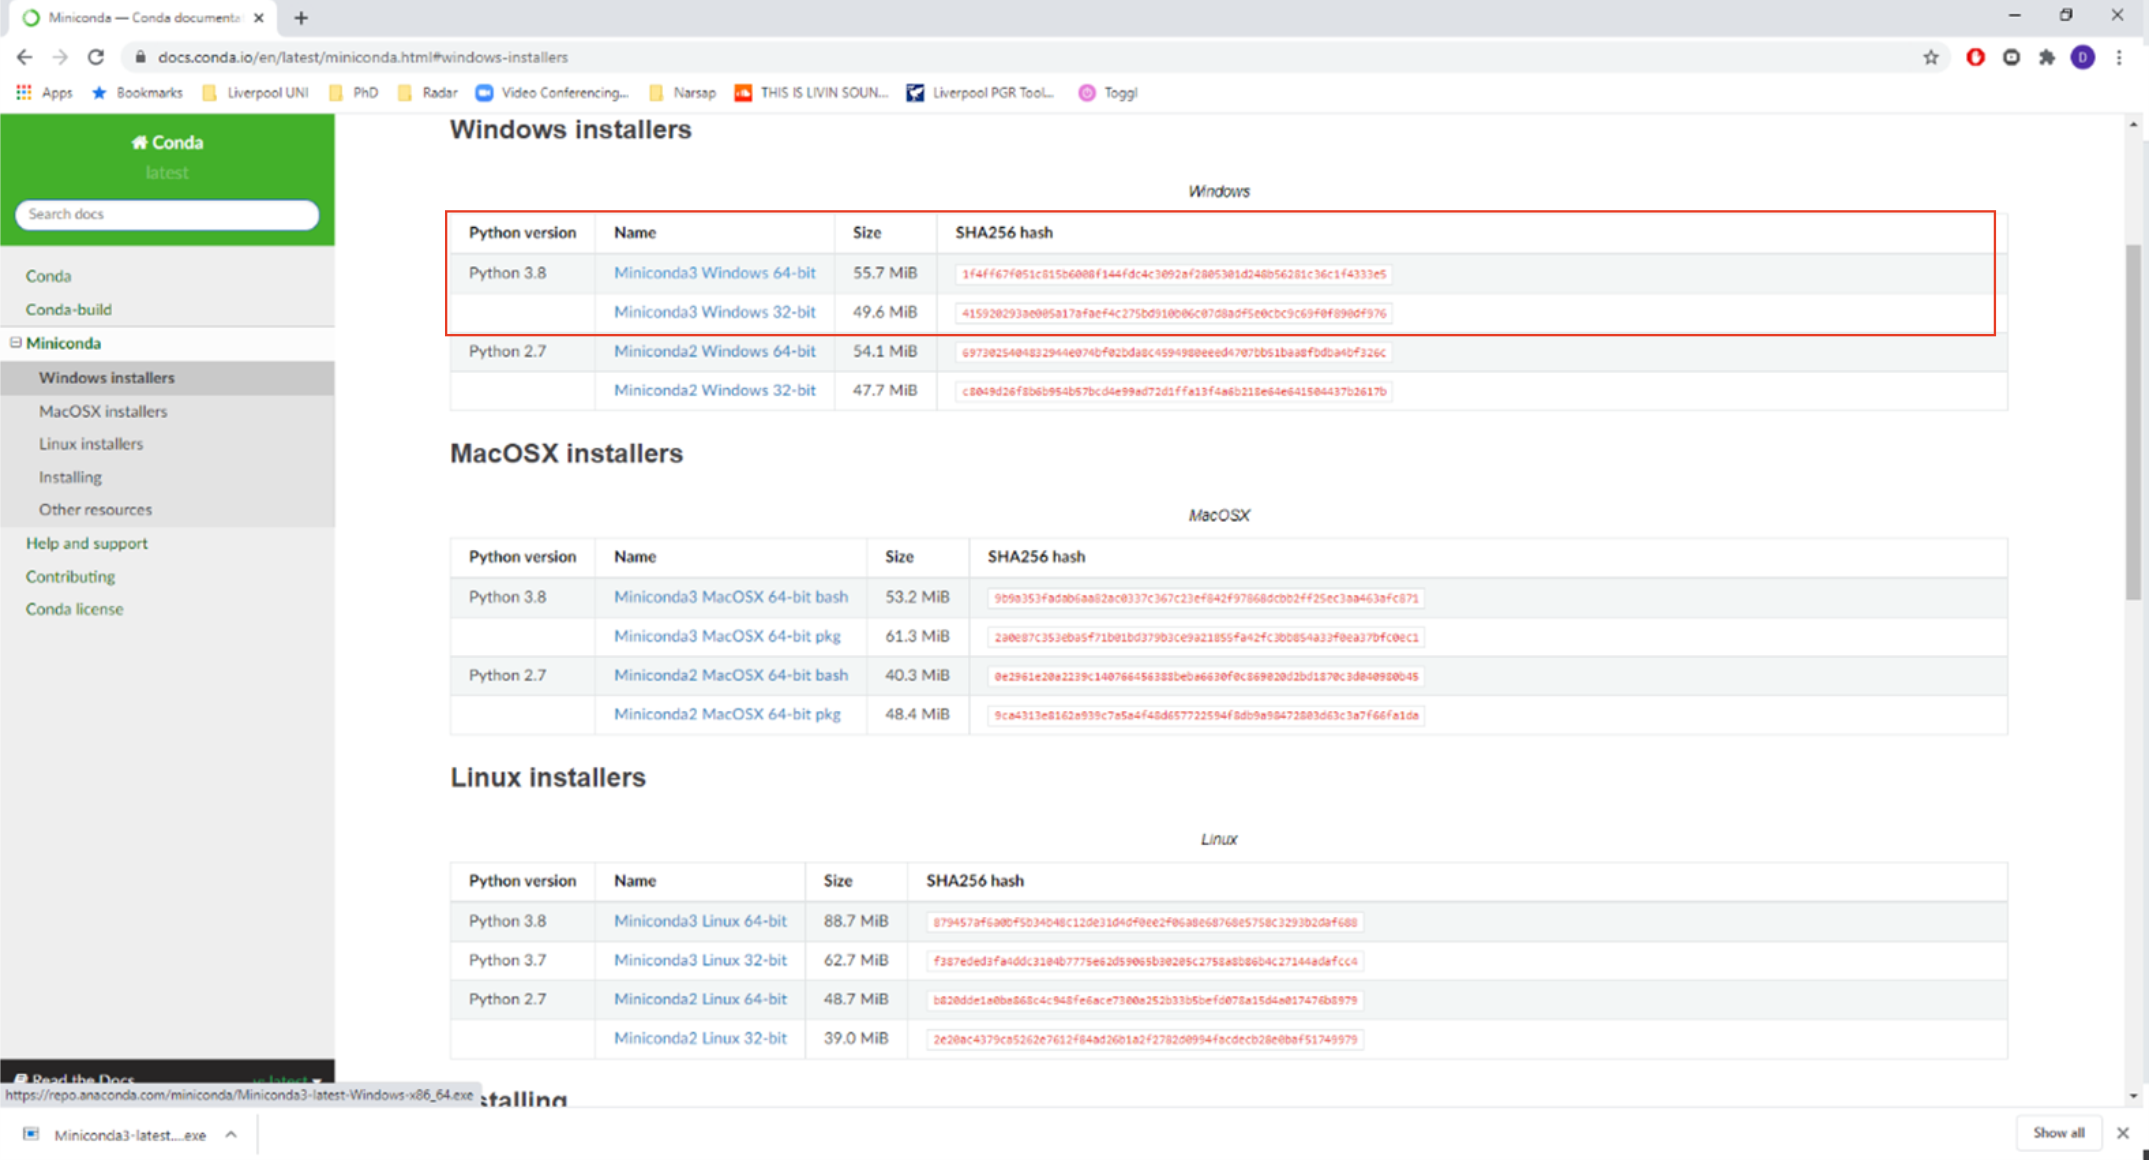
\includegraphics[width=29.86in]{figs/chp4/Picture10} \end{center}

\begin{itemize}
\tightlist
\item
  This will bring you to the \href{https://docs.conda.io/en/latest/miniconda.html\#windows-installers}{Miniconda download} page shown above.
\item
  You have installation files for two different Python version (2.7 and 3.8) and for two different Windows systems (32 bit and 64 bit).
\item
  We are using \textbf{Python 3.8}, so depending on which windows version you are using (32-bit or 64-bit), click on the relevant file in the Python 3.8 section (highlighted in red).
\item
  This will download the Miniconda installation file to your \textbf{Downloads folder}.
\end{itemize}

\begin{center}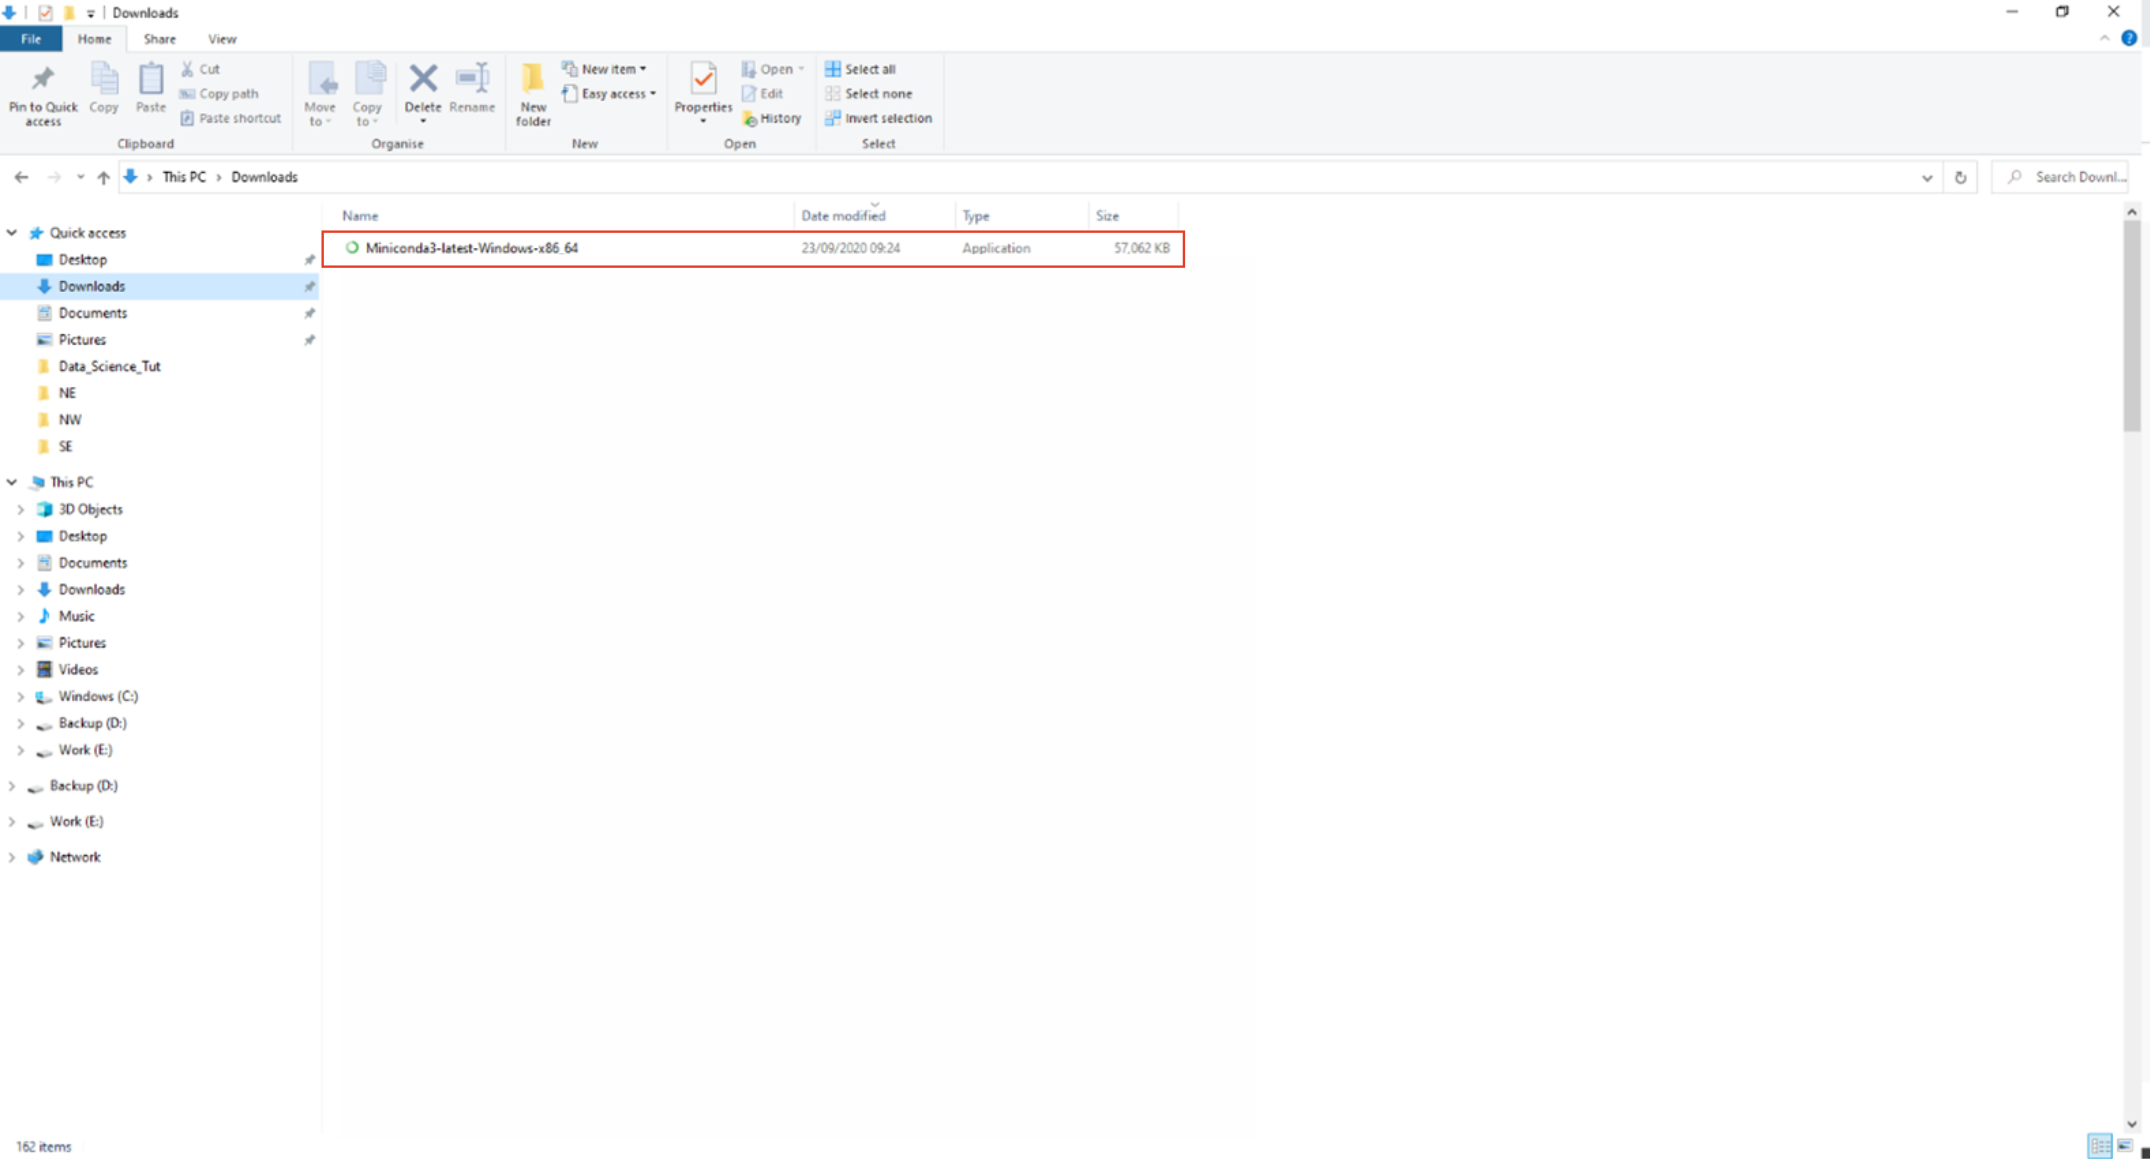
\includegraphics[width=29.86in]{figs/chp4/Picture11} \end{center}

\begin{itemize}
\tightlist
\item
  Once the download has finished,navigate to your \textbf{Downloads folder} on your computer and double click on the \emph{Miniconda3-latest-Windows-x86\_64} file to start the installation.
\item
  Note: Double-check that you are installing the right version for your system.
\end{itemize}

\hypertarget{installing-minicoda}{%
\subsection*{Installing Minicoda}\label{installing-minicoda}}
\addcontentsline{toc}{subsection}{Installing Minicoda}

\begin{center}\includegraphics[width=7.22in]{figs/chp4/Inst_1} \end{center}

\begin{itemize}
\tightlist
\item
  Double clicking the downloaded file will open an installation window.
\item
  Click \textbf{\emph{Next}} on the first step.
\end{itemize}

\begin{center}\includegraphics[width=7.24in]{figs/chp4/Inst_2} \end{center}

\begin{itemize}
\tightlist
\item
  Click \textbf{\emph{I Agree}} in the next step which is the Terms and Conditions.
\end{itemize}

\begin{center}\includegraphics[width=7.15in]{figs/chp4/Inst_3} \end{center}

\begin{itemize}
\tightlist
\item
  In the next window, you can select if you want to install Miniconda for all users or just you.
\item
  Check that \textbf{\emph{Just Me}} is selected and click next.
\end{itemize}

\begin{center}\includegraphics[width=7.17in]{figs/chp4/Inst_4} \end{center}

\begin{itemize}
\tightlist
\item
  The next window will ask you where to install Miniconda.
\item
  Leave the path (highlighted in blue) as is and click next.
\end{itemize}

\begin{center}\includegraphics[width=7.18in]{figs/chp4/Inst_5} \end{center}

\begin{itemize}
\tightlist
\item
  The next window can be used for an advanced setup
\item
  Leave the default settings as they are (Box ticked at \emph{Register Miniconda3 as my default Python 3.8}).
\end{itemize}

\begin{center}\includegraphics[width=7.17in]{figs/chp4/Inst_6} \end{center}

\begin{itemize}
\tightlist
\item
  Miniconda is now installing.
\item
  Once the installation is complete, click \textbf{\emph{Next}}.
\end{itemize}

\begin{center}\includegraphics[width=7.15in]{figs/chp4/Inst_7} \end{center}

• Untick all boxes in the window (unless you want further information on Miniconda, which will open in your browser) and click \textbf{\emph{Finish}}.

\hypertarget{running-minicoda}{%
\subsection*{Running Minicoda}\label{running-minicoda}}
\addcontentsline{toc}{subsection}{Running Minicoda}

\begin{center}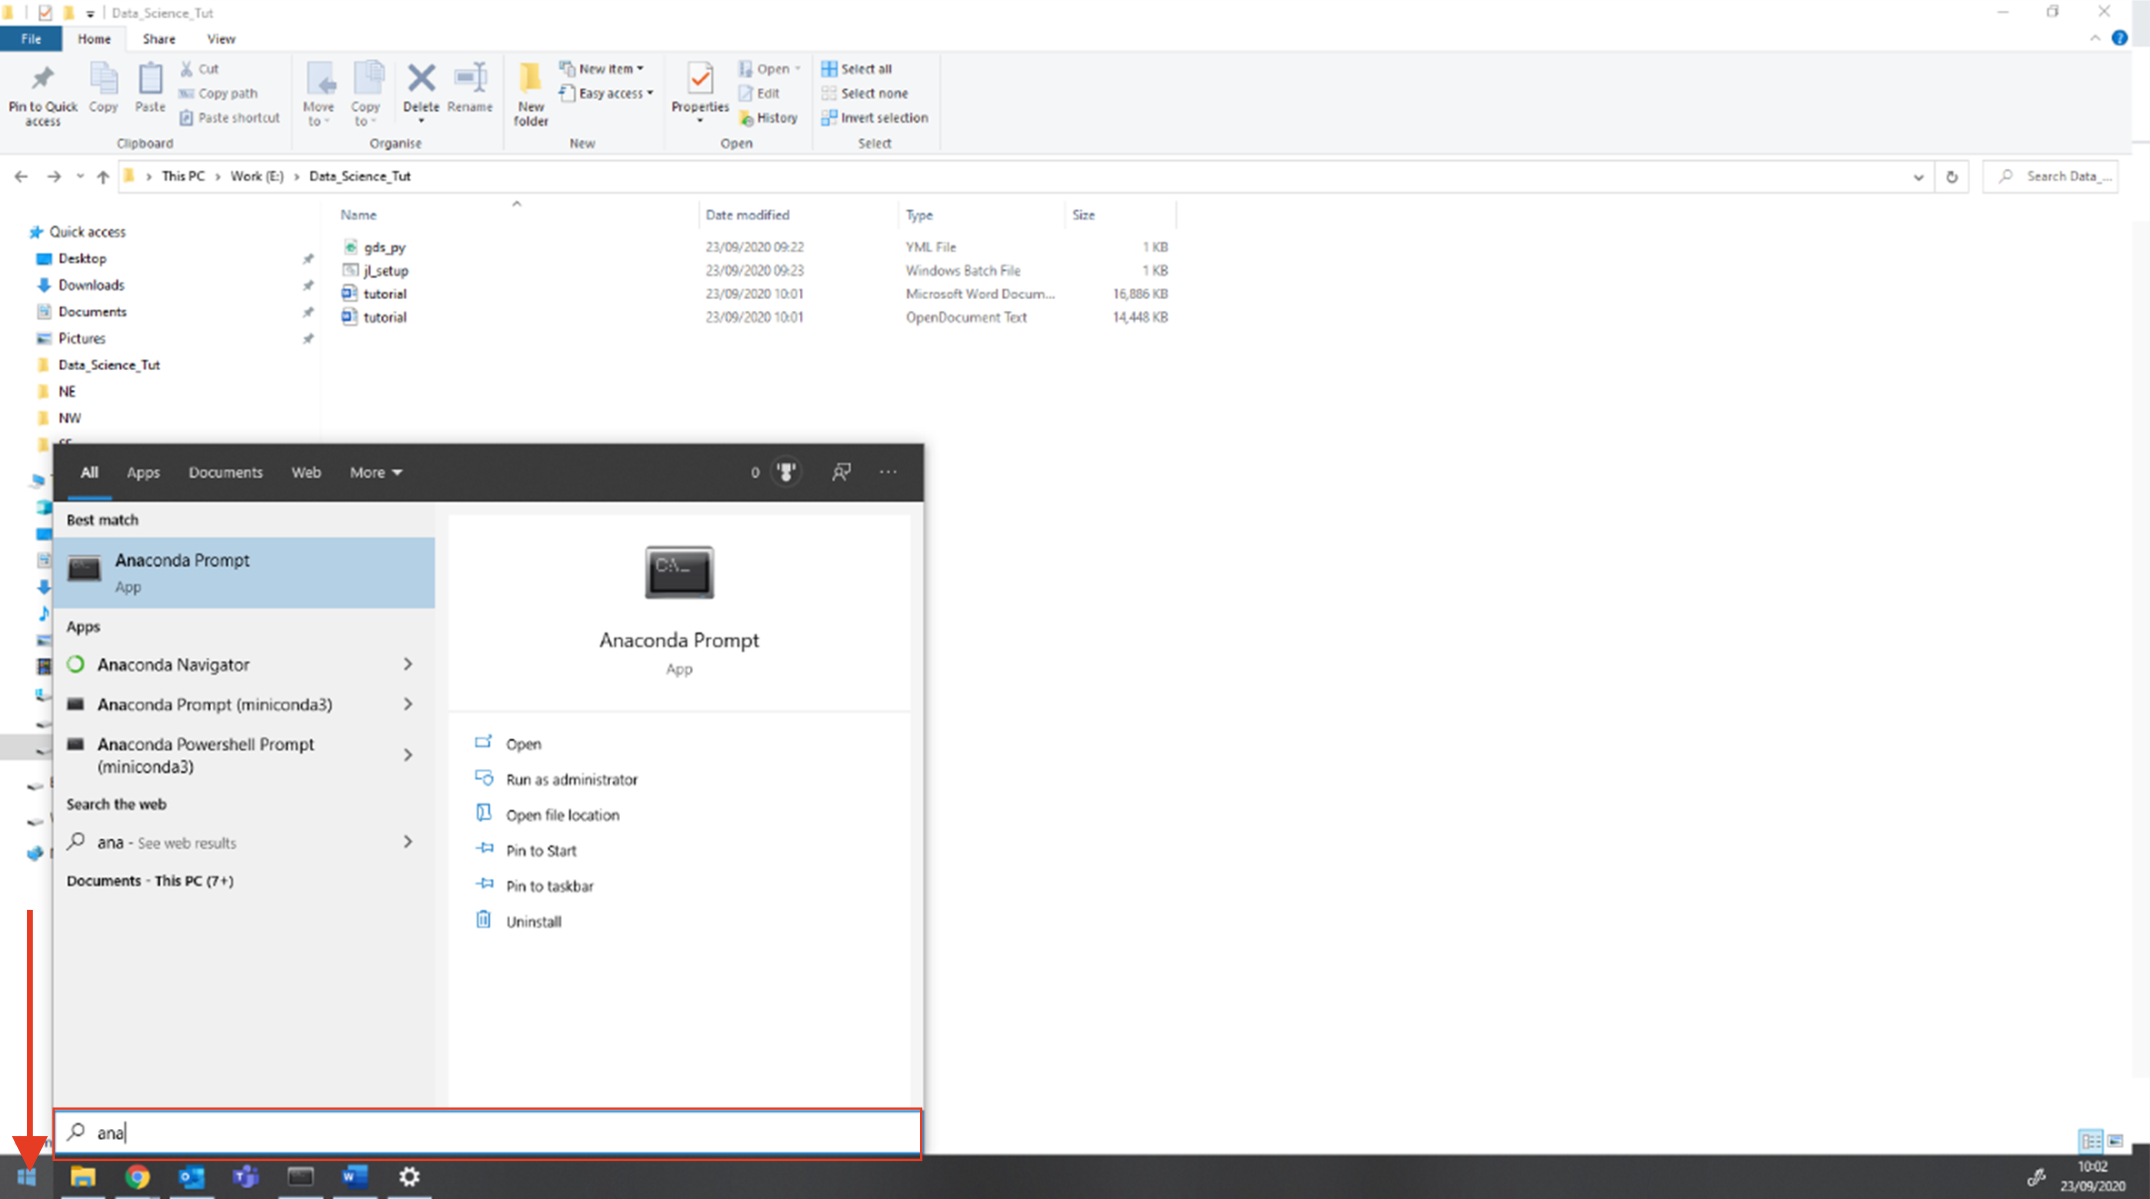
\includegraphics[width=29.86in]{figs/chp4/Picture20} \end{center}

\begin{itemize}
\tightlist
\item
  Open Miniconda by clicking on the Windows icon on the bottom left of your screen and either type \textbf{\emph{Anaconda}} or look for the \textbf{Anaconda folder} in the menu.
\end{itemize}

\begin{center}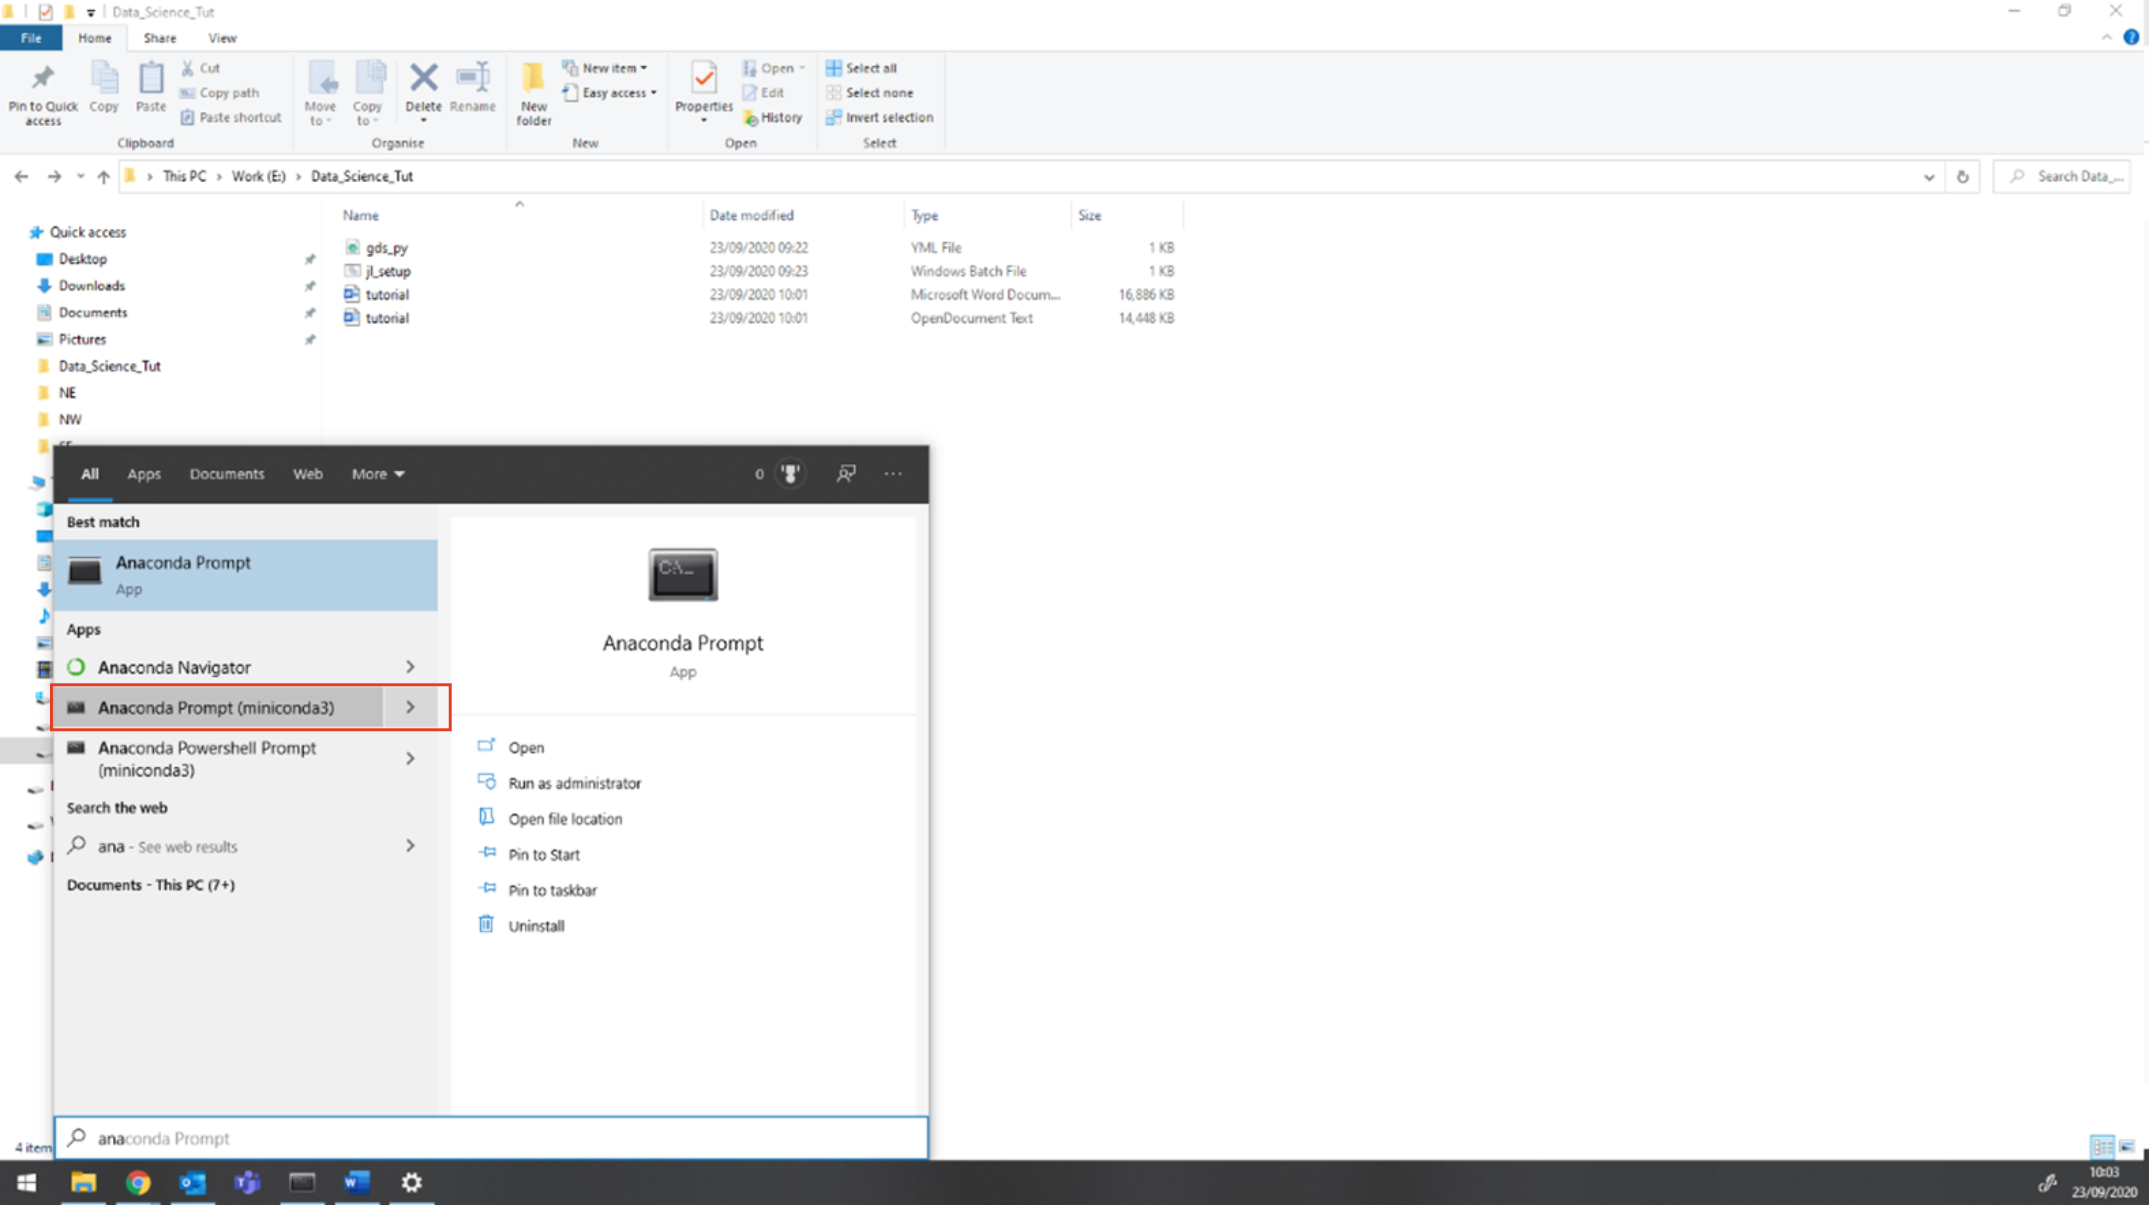
\includegraphics[width=29.85in]{figs/chp4/Picture21} \end{center}

\begin{itemize}
\tightlist
\item
  To open Miniconda, click on \textbf{\emph{Anaconda Prompt (miniconda3)}}.
  \textbf{Note:} From now on we will refer to the prompt as \textbf{Anaconda Prompt}
\end{itemize}

\begin{center}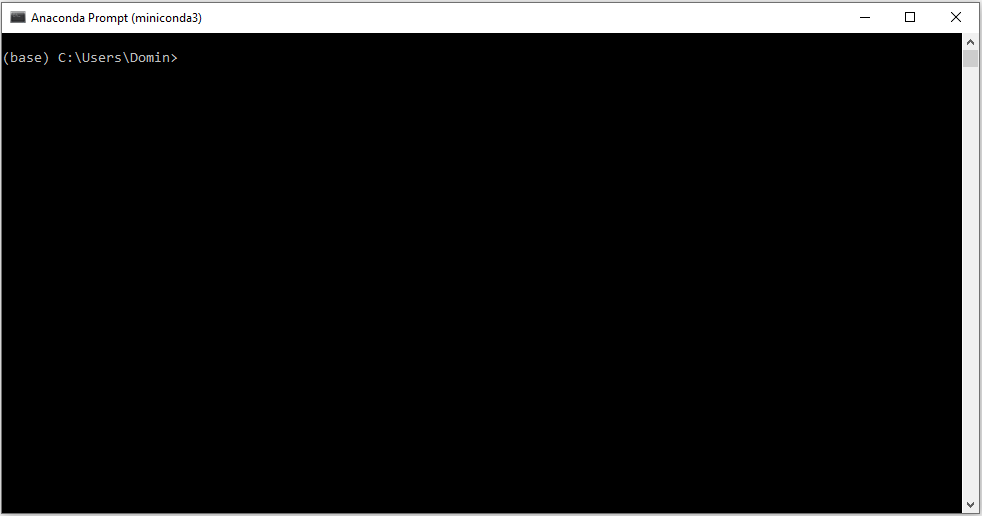
\includegraphics[width=13.64in]{figs/chp4/Conda_1} \end{center}

\begin{itemize}
\tightlist
\item
  This will open the Anaconda command prompt.
\end{itemize}

\begin{center}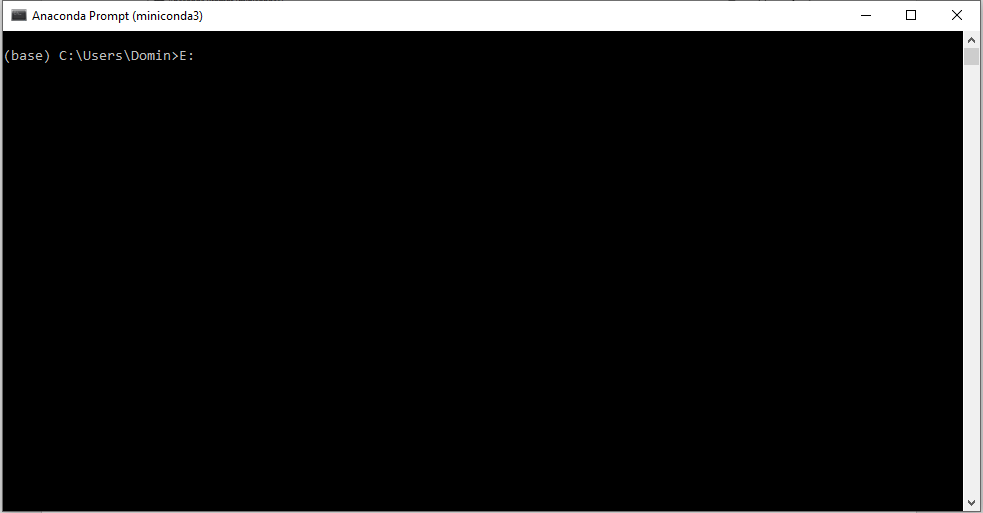
\includegraphics[width=13.65in]{figs/chp4/Conda_2} \end{center}

\begin{center}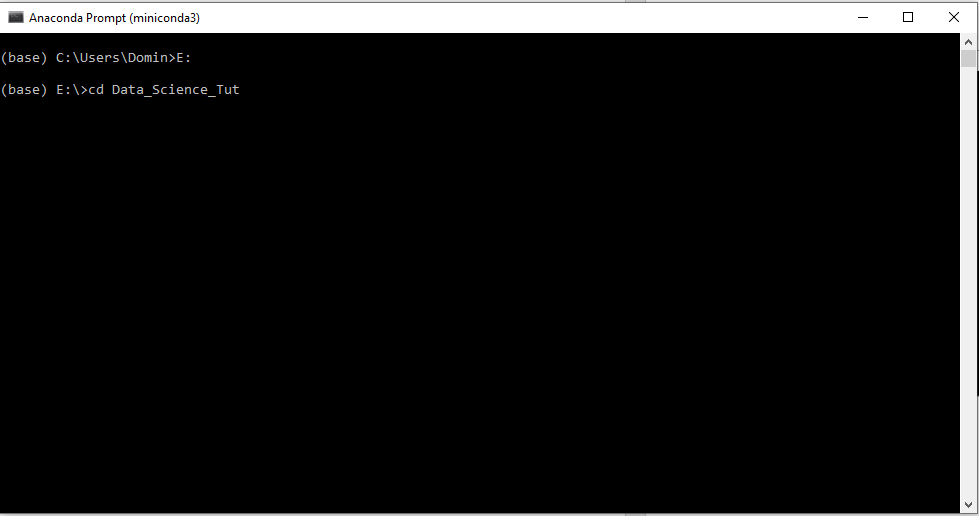
\includegraphics[width=13.6in]{figs/chp4/Conda_3} \end{center}

\begin{itemize}
\item
  You now need to navigate to the folder that contains your environment (\texttt{\_gds\_py.yml\_}) and setup (\texttt{\_jl\_setup.bat\_}) files.
\item
  you can move to the folder by running \texttt{cd} to move forward through folders and \texttt{cd\ ..} to move backwards.
\item
  To run a command you simply press enter.
\item
  If your files are stored in e.g.~C:/Users/Domin/Desktop/GDS\_2020 you would write \texttt{cd\ Desktop/GDS\_2020}
\item
  If your files are stored in a different location e.g.~E:/Data\_science\_Tut, you would run \texttt{E:}
  (to switch the harddrive) followed by \texttt{cd\ Data\_science\_Tut}.
\end{itemize}

\begin{center}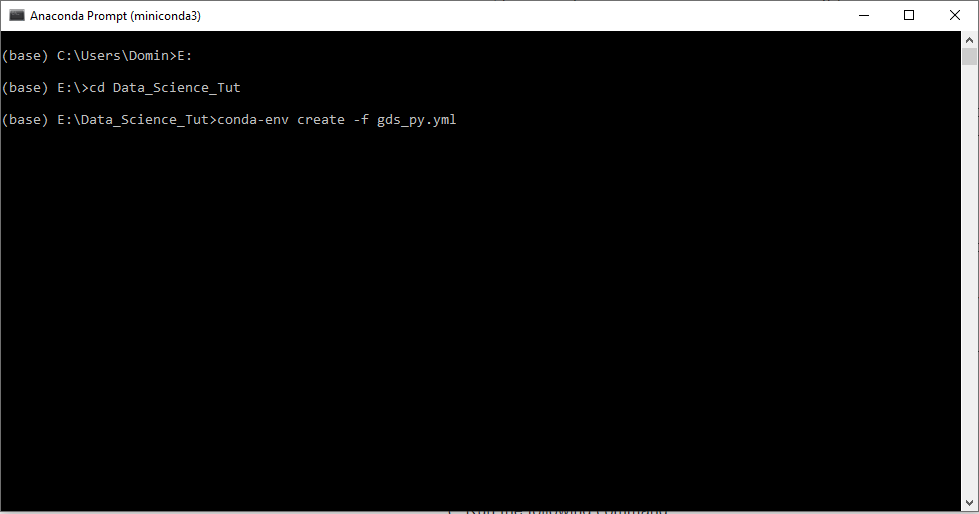
\includegraphics[width=13.6in]{figs/chp4/Conda_4} \end{center}

\begin{itemize}
\tightlist
\item
  Once you have navigated to the location of your files, write the following in the Anaconda prompt and press enter to run it.
\end{itemize}

\texttt{conda-env\ create\ -f\ gds\_py.yml}

\begin{itemize}
\tightlist
\item
  This will install all packages that are required to complete the course and setup your Python environment.
  ** Note: This might take a while as it is downloading all packages (\textasciitilde{} 500 MB).**
\end{itemize}

\begin{center}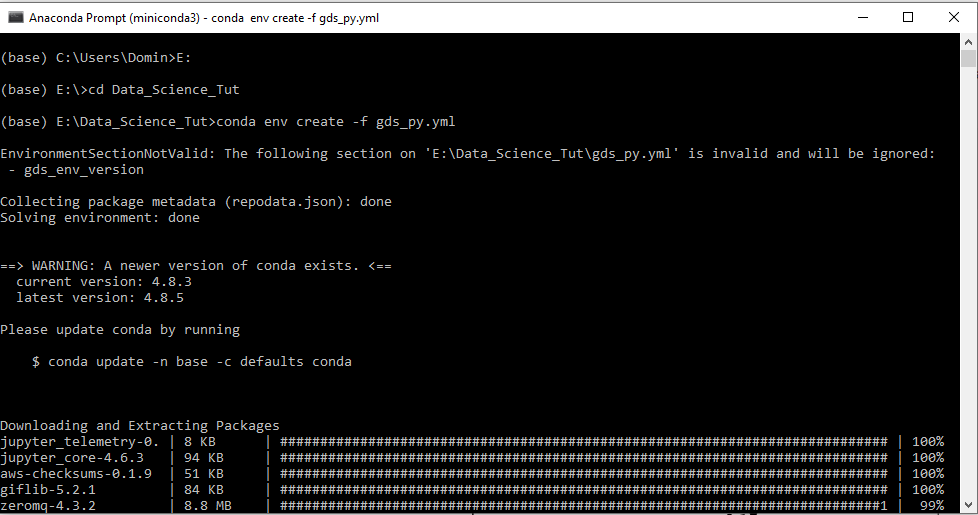
\includegraphics[width=13.58in]{figs/chp4/Conda_6} \end{center}

\begin{itemize}
\tightlist
\item
  The packages that are being installed will be shown in the Anaconda prompt.
\end{itemize}

\begin{center}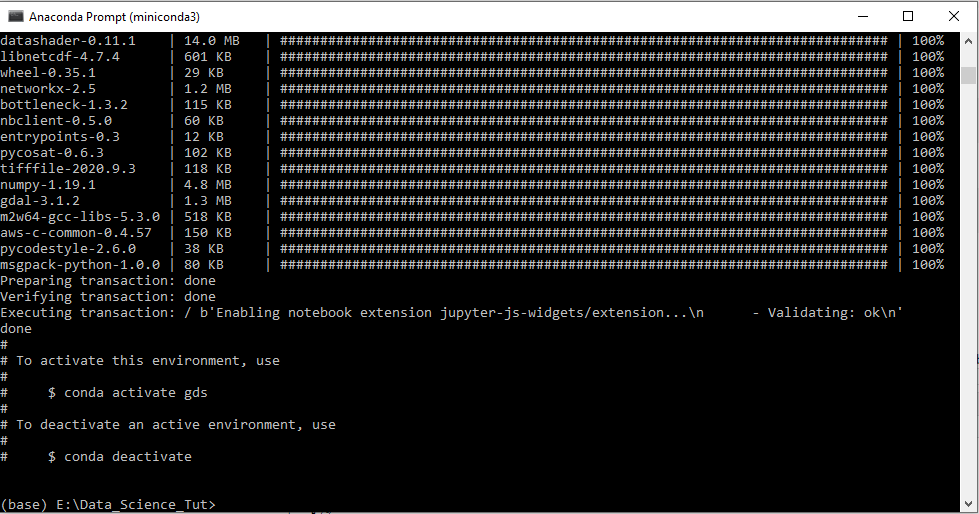
\includegraphics[width=13.6in]{figs/chp4/Conda_7} \end{center}

\begin{itemize}
\tightlist
\item
  Once all packages have been installed and your environment is created, you can activate the environment with the following command:
\end{itemize}

\texttt{conda\ activate\ gds}

\hypertarget{complete-environment-setup}{%
\subsection{Complete environment Setup}\label{complete-environment-setup}}

We will now complete the setup by installing the user interface (Jupyter Lab) which you will need to code.

\begin{center}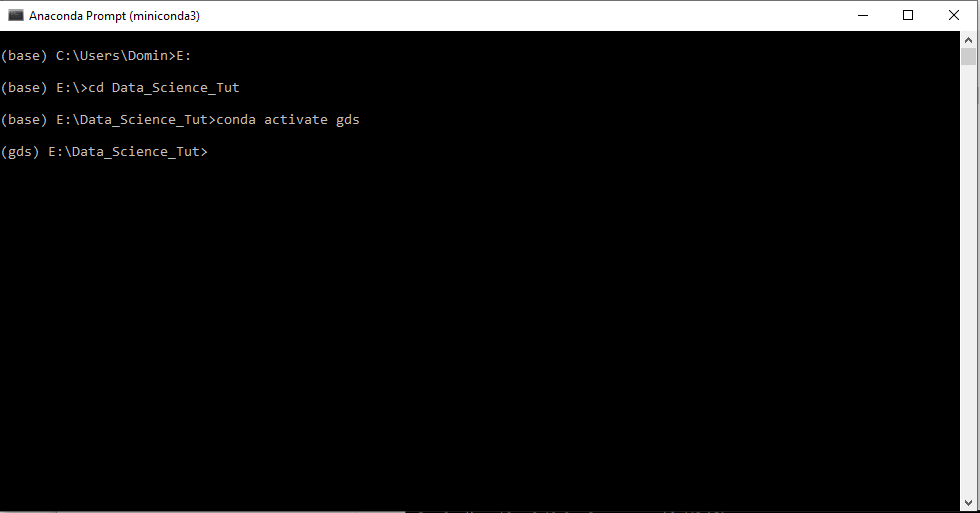
\includegraphics[width=13.61in]{figs/chp4/Conda_8} \end{center}

\begin{itemize}
\tightlist
\item
  Activate the environment by running :
\end{itemize}

\texttt{conda\ activate\ gds}

\begin{itemize}
\tightlist
\item
  You can see that the start of the line has changed from \textbf{(base)} to \textbf{(gds)}.
\end{itemize}

\begin{center}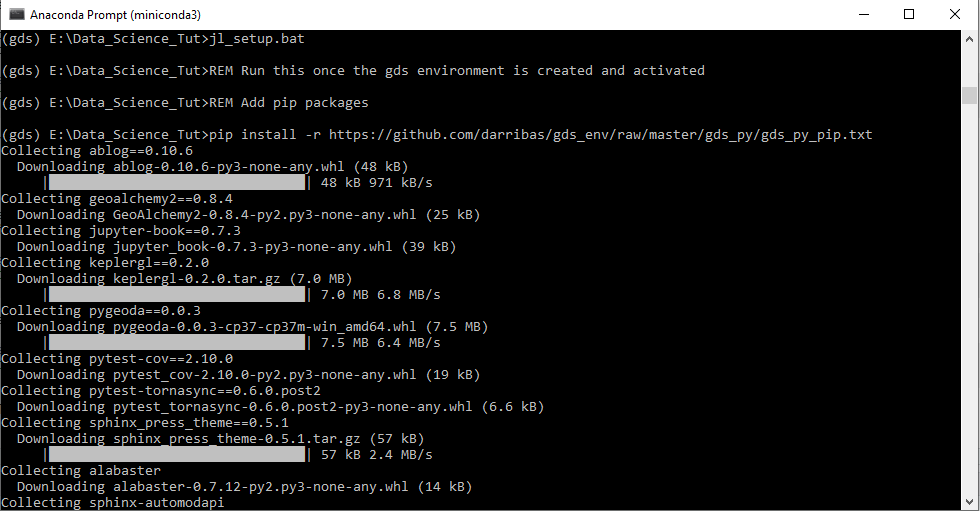
\includegraphics[width=13.61in]{figs/chp4/Conda_9} \end{center}

\begin{itemize}
\tightlist
\item
  In the same prompt, run the following command to complete the environment setup
\end{itemize}

\texttt{jl\_setup.bat}

\begin{itemize}
\tightlist
\item
  The prompt will show you the further packages that are being installed.
\end{itemize}

\textbf{NOTE:} This might take a while depending on your internet connection (at least 10-15 minutes).
\textbf{NOTE:} Do not close the Anaconda prompt yet as we will need it again.

\hypertarget{check-installation}{%
\subsection{Check Installation}\label{check-installation}}

To make sure that your installation was successful and all packages have been installed we need to run one more step.

\begin{center}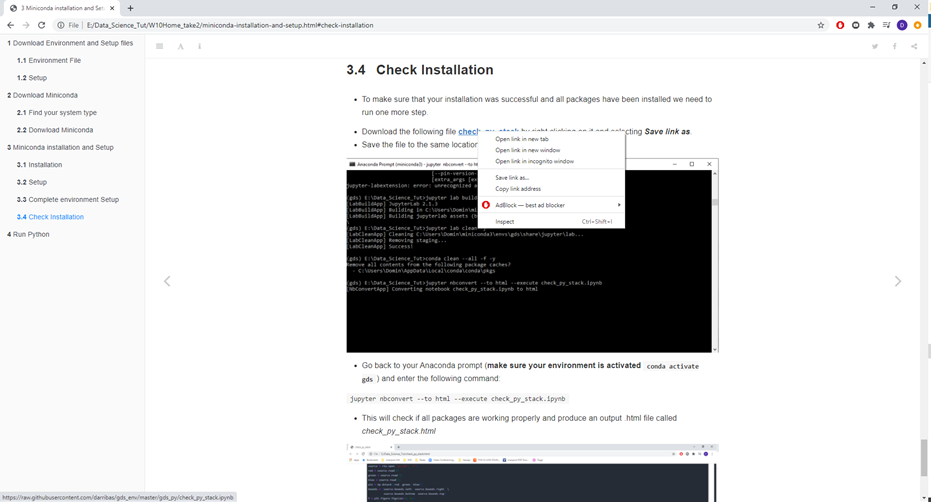
\includegraphics[width=12.93in]{figs/chp4/Picture22} \end{center}

\begin{itemize}
\tightlist
\item
  Download the following file \href{https://raw.githubusercontent.com/darribas/gds_env/master/gds_py/check_py_stack.ipynb}{\textbf{check\_py\_stack}} by right clicking on it and selecting \textbf{\emph{Save link as}}.
\item
  Save the file to the same location as all other files.
\end{itemize}

\begin{center}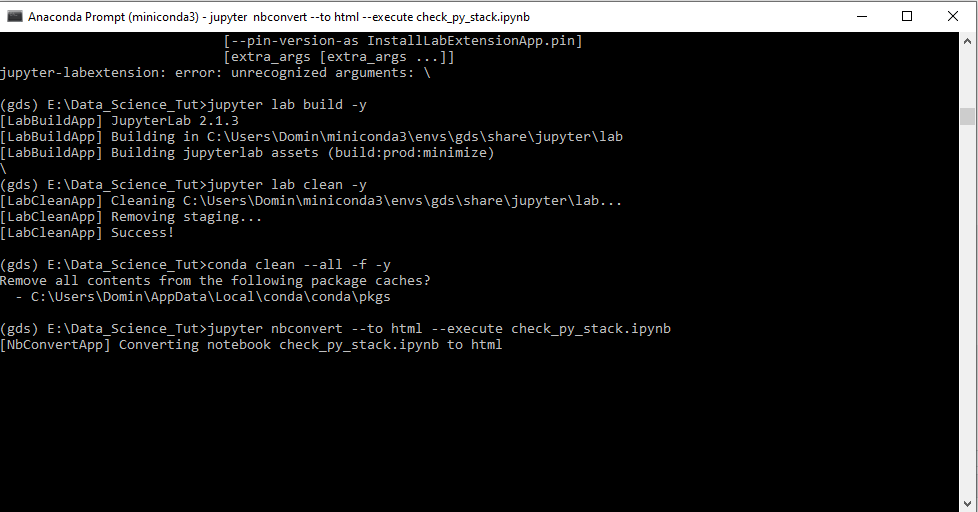
\includegraphics[width=13.58in]{figs/chp4/Conda_11} \end{center}

\begin{itemize}
\tightlist
\item
  Go back to your Anaconda prompt (\textbf{make sure your environment is activated \texttt{conda\ activate\ gds} }) and enter the following command:
\end{itemize}

\texttt{jupyter\ nbconvert\ -\/-to\ html\ -\/-execute\ check\_py\_stack.ipynb}

\begin{itemize}
\tightlist
\item
  This will check if all packages are working properly and produce an output \texttt{.html} file called \emph{check\_py\_stack.html}
\end{itemize}

\begin{center}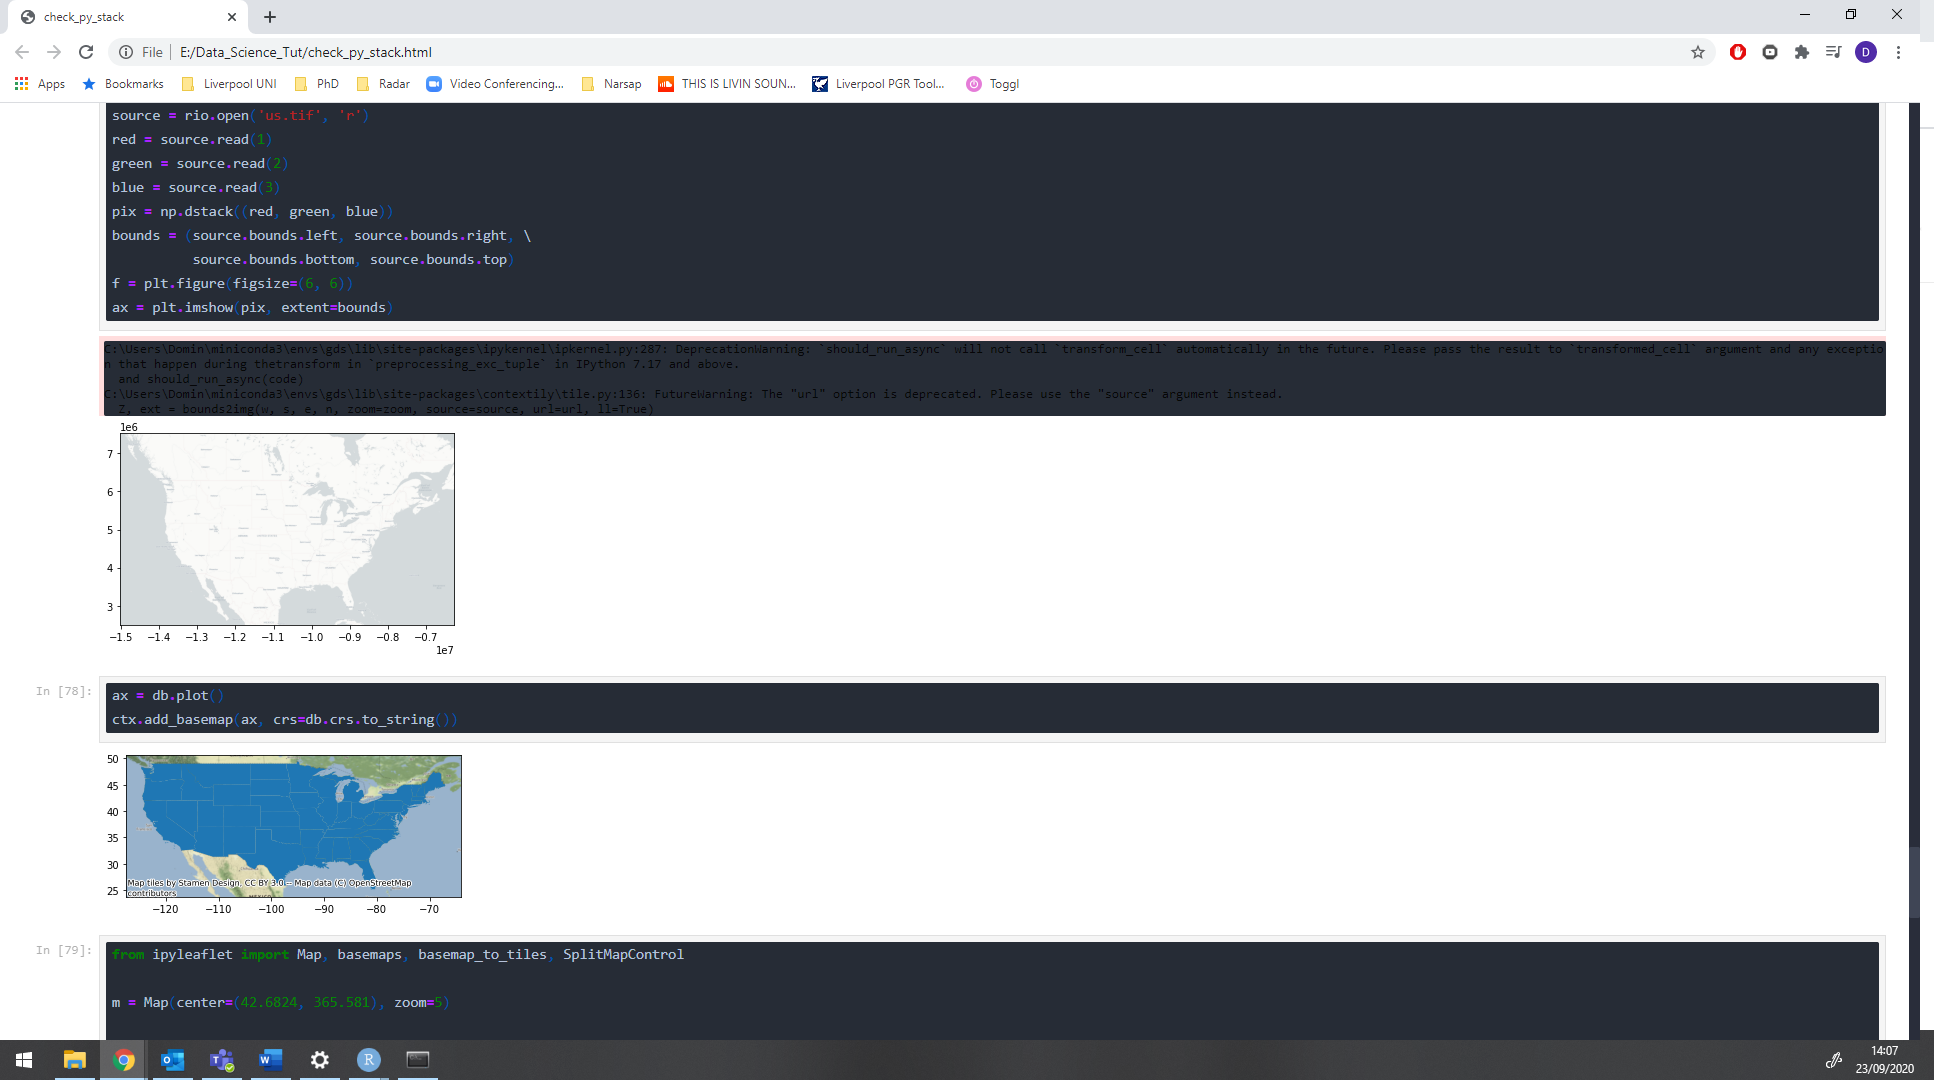
\includegraphics[width=26.86in]{figs/chp4/Picture23} \end{center}

\begin{itemize}
\tightlist
\item
  Double clicking on the \emph{check\_py\_stack.html} file will open the file in a browser and you can check if the code has produce an output in all cells.
\end{itemize}

\hypertarget{running-python}{%
\section*{Running Python}\label{running-python}}
\addcontentsline{toc}{section}{Running Python}

Now that you have successfully installed Python/Anaconda, you are ready to start coding.
To launch your coding environment complete the following steps:

\begin{enumerate}
\def\labelenumi{\arabic{enumi}.}
\item
  Start by opening an Anaconda Prompt (see first steps of section 3.2 on how to open an Anaconda prompt).
\item
  Navigate to the folder that you want to work in (It is recommended to have all your files in one folder with subfolders) using the \texttt{cd} command.
\item
  Activate your environment by running \texttt{conda\ activate\ gds}.
\end{enumerate}

\begin{center}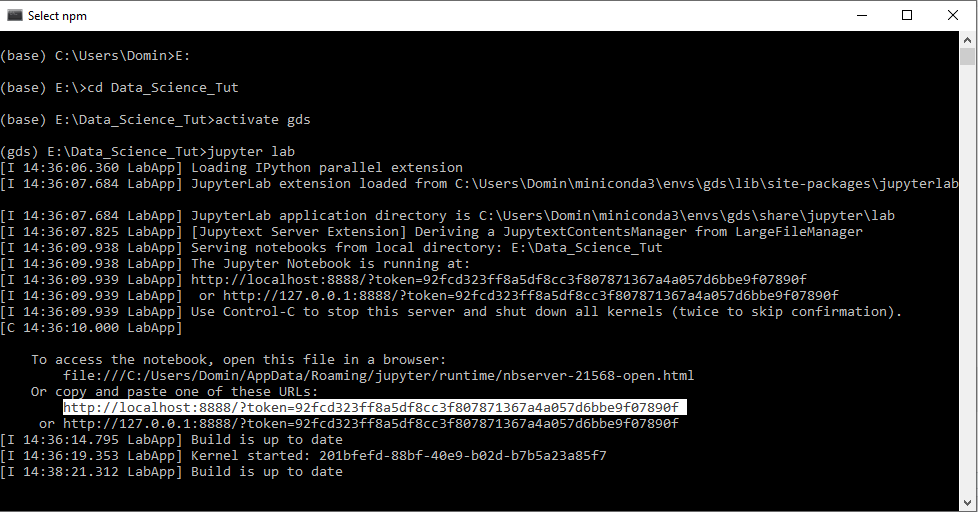
\includegraphics[width=13.58in]{figs/chp4/Conda_13} \end{center}

\begin{enumerate}
\def\labelenumi{\arabic{enumi}.}
\setcounter{enumi}{3}
\tightlist
\item
  Run the command \texttt{jupyer\ lab} to start your coding interface. The coding interface will launch in your default browser (We recommend using Chrome or Firefox).
\end{enumerate}

If your default browser is neither of the recommended, you can close the window that opens automatically, open Chrome/Firefox and past the URL from the Anaconda Prompt.

\begin{center}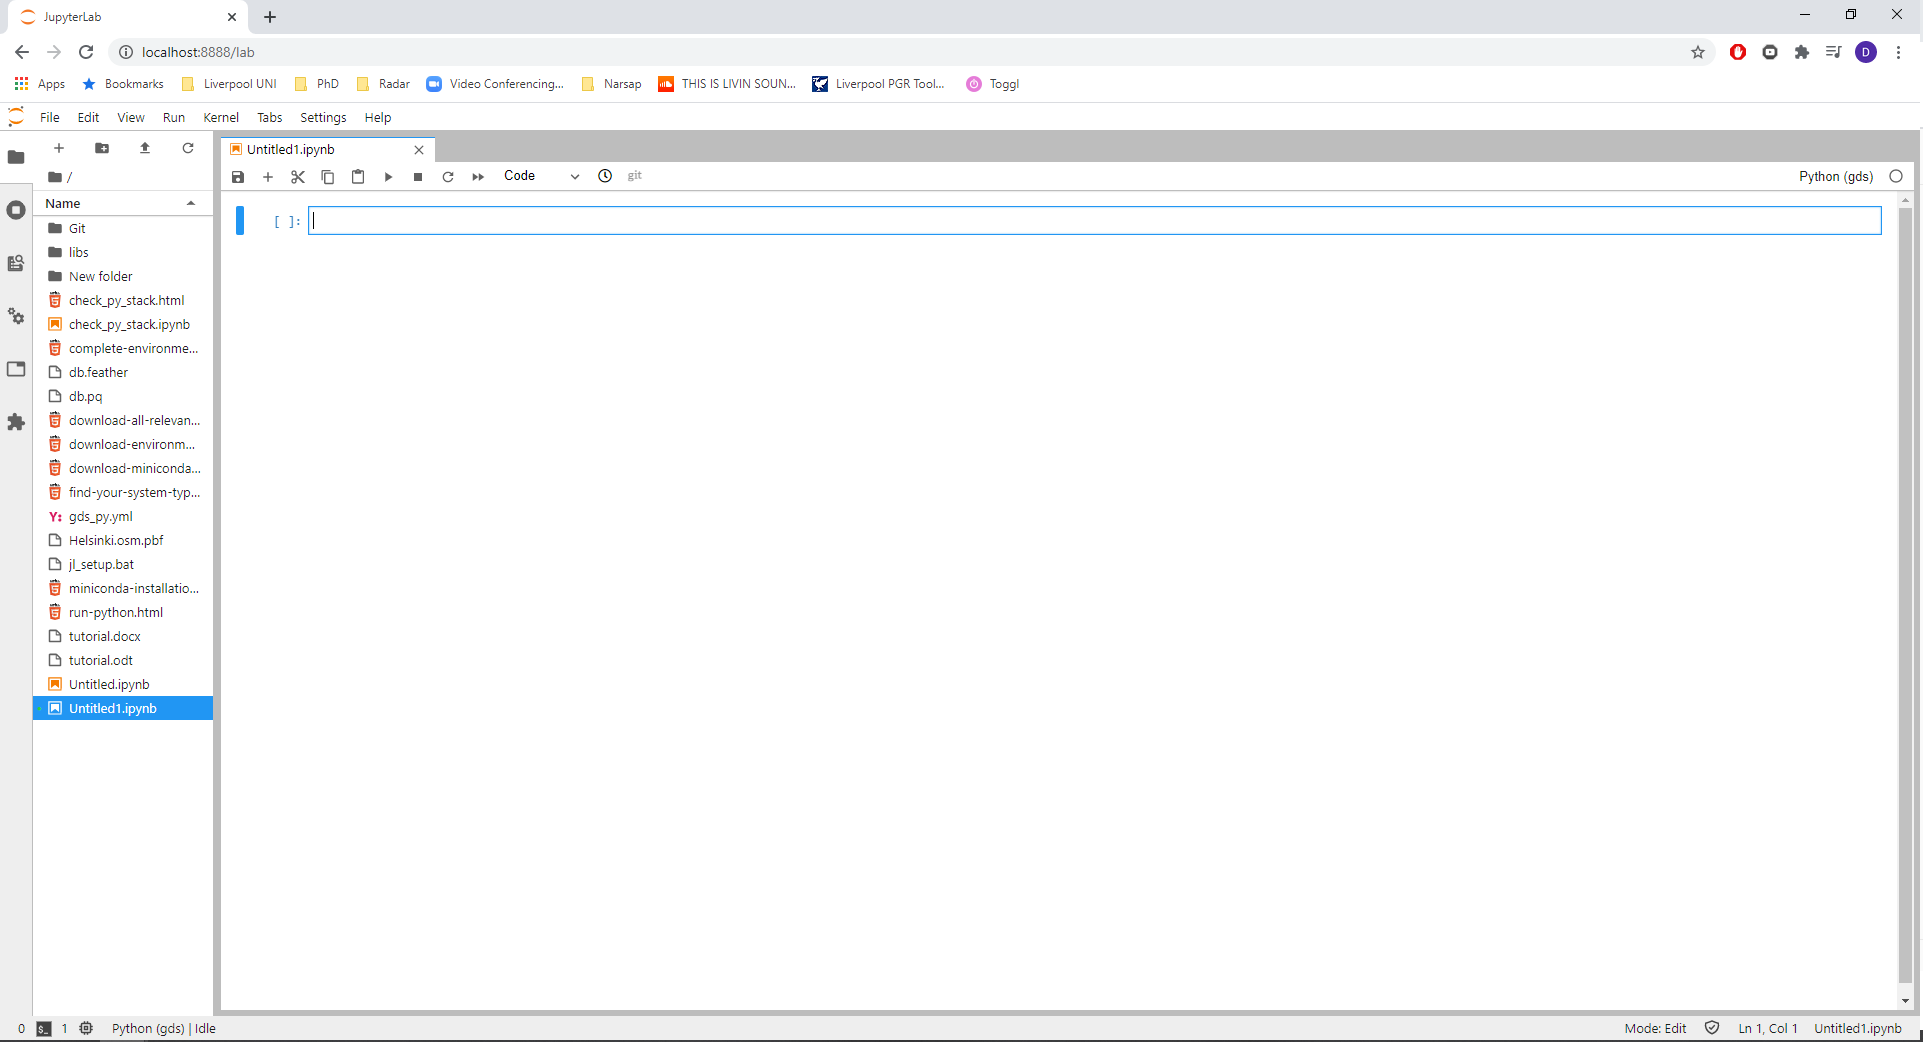
\includegraphics[width=26.71in]{figs/chp4/Picture24} \end{center}

\begin{enumerate}
\def\labelenumi{\arabic{enumi}.}
\setcounter{enumi}{4}
\tightlist
\item
  Jupyter Lab (your coding interface) will open automatically.
\end{enumerate}

\textbf{CONGRATULATIONS YOU HAVE NOW SUCCESFULLY INSTALLED PYTHON}

\textbf{You can now start coding}

\includegraphics{https://media.giphy.com/media/PiQejEf31116URju4V/giphy.gif}

\hypertarget{windows-version}{%
\chapter*{Windows Version}\label{windows-version}}
\addcontentsline{toc}{chapter}{Windows Version}

Find your Windows version

\begin{center}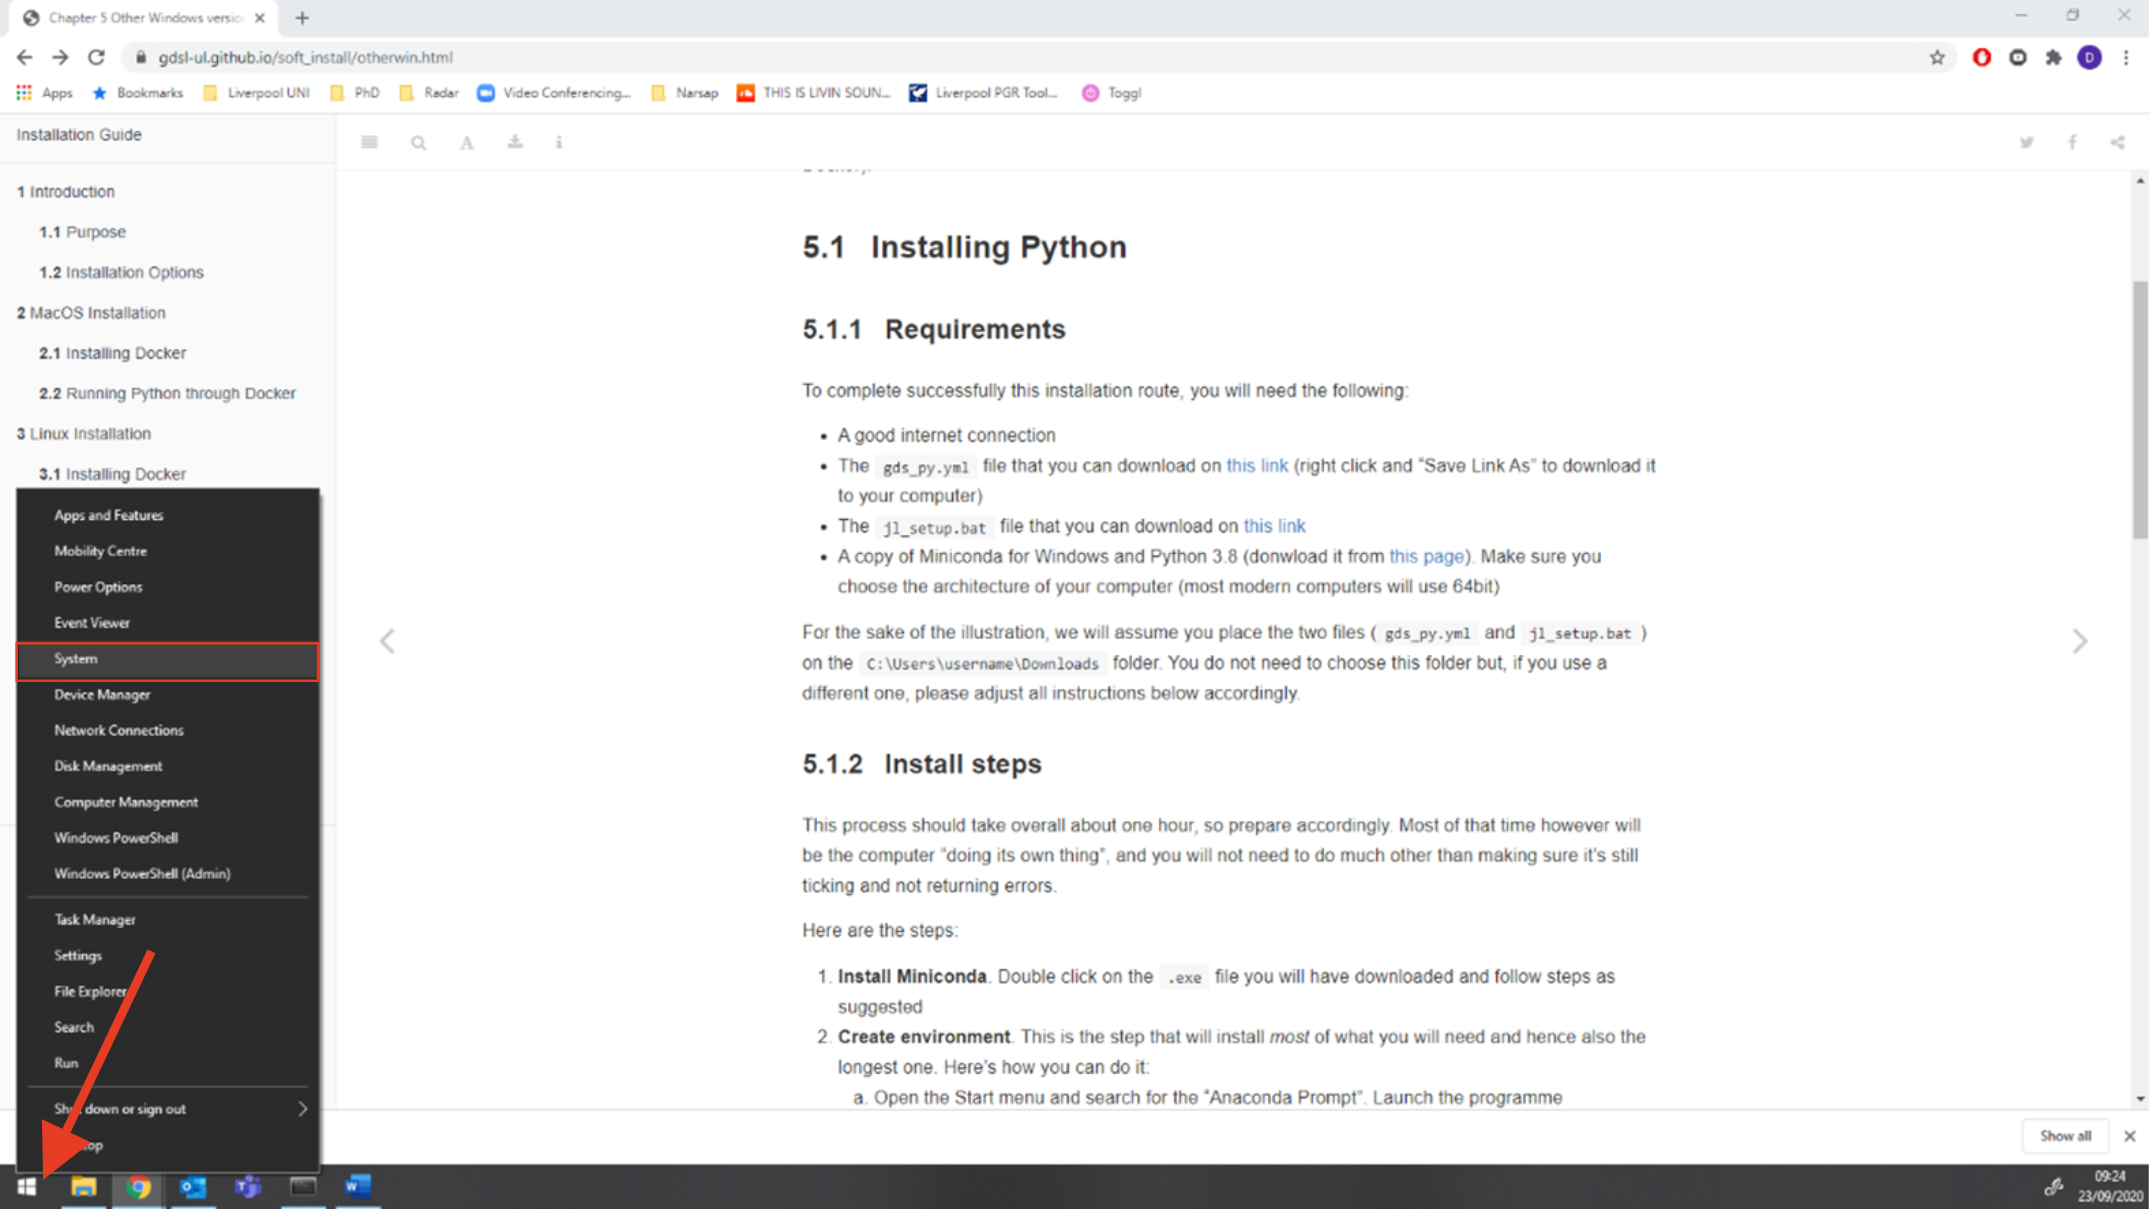
\includegraphics[width=29.85in]{figs/chp5/Picture7} \end{center}

\begin{itemize}
\tightlist
\item
  Right click on the Windows logo in the left bottom corner of your screen and click on \emph{system}.
\end{itemize}

\begin{center}\includegraphics[width=67.29in]{figs/chp5/Version_tut_1} \end{center}

\begin{itemize}
\tightlist
\item
  You can find your Windows version under \emph{Windows Specifications} and \emph{Edition} (Here it is Windows 10 Home).
\end{itemize}

  \bibliography{book.bib,packages.bib}

\end{document}
